%%%%%%%%%%%%%%%%%%%%%%%%%%%%%%%%%%%%%%%%%%%%%%%%%%%%%%%
% A template for Wiley article submissions.
% Developed by Overleaf. 
%
% Please note that whilst this template provides a 
% preview of the typeset manuscript for submission, it 
% will not necessarily be the final publication layout.
%
% Usage notes:
% The "blind" option will make anonymous all author, affiliation, correspondence and funding information.
% Use "num-refs" option for numerical citation and references style.
% Use "alpha-refs" option for author-year citation and references style.

\documentclass[alpha-refs]{wiley-article-01g}
% \documentclass[blind,num-refs]{wiley-article}

% Add additional packages here if required
\usepackage{siunitx}

% For figures

\usepackage{graphics}

%For captions 
\usepackage[labelfont=bf,justification=centering]{caption}
\usepackage[font=small,labelfont=bf]{subcaption}
\captionsetup[sub]{font=tiny,labelfont={bf,sf}}

%% For figures numbered by section
\usepackage{chngcntr}
\counterwithin{figure}{section}
\counterwithin{table}{section}

%% Additional links for hyperref
\usepackage[unicode=true,pdfusetitle,
 bookmarks=true,bookmarksnumbered=true,bookmarksopen=true,bookmarksopenlevel=2,
 breaklinks=false,pdfborder={0 0 1},backref=false,colorlinks=false]
 {hyperref}
\hypersetup{pdfstartview={XYZ null null 1}}


%% For fillers
\usepackage{lipsum}

%% For references 
\usepackage[backend=bibtex,
			natbib=true, 
			style=chicago-authordate]{biblatex}
\addbibresource{Returns.bib}

%% For landscape pages 

\usepackage{lscape}

%%%%%%%%#################################################################################%%%%%%%%%%%%%%%%%%%%%%%%%%%%%

% Update article type if known
\papertype{WORLD BANK EDUCATION GLOBAL PRACTICE}
% Include section in journal if known, otherwise delete
\paperfield{Russian Federation: Analytical Services and Advisory Activity: 
P170978}

\title{Returns to Education in the Russian Federation: Some New Estimates}

% List acknowledgements here.
\fundinginfo{Thanks are due to the Higher School of Economics, Moscow for making the Russian Longitudinal Monitoring Study (RLMS) Household data readily available for reseachers around the world. The code used for this paper is made freely available for all researchers at \url{https://bitbucket.org/zagamog/edreru/src/master/}}

% Include full author names and degrees, when required by the journal.
% Use the \authfn to add symbols for additional footnotes and present addresses, if any. Usually start with 1 for notes about author contributions; then continuing with 2 etc if any author has a different present address.

\author[1]{Harry Patrinos}
\author[2]{\hspace{-1em}Suhas Parandekar}
\author[3]{\hspace{-1em}Ekaterina Melianova}
\author[4]{\hspace{-1em}Art\"{e}m Volgin}

% List abbreviations here, if any. Please note that it is preferred that abbreviations be defined at the first instance they appear in the text, rather than creating an abbreviations list.
\acks{\begin{normalsize}
\emph{Country Director:} Renaud Seligman; \emph{Regional Director:} Fadia Saadah; \emph{Practice Manager:} Harry Patrinos; \emph{Program Leader:} Dorota Nowak; \emph{Peer Reviewers}: Cristian Aedo; Ruslan Yemtsov; Husein Abdul-Hamid; \emph{Team members:} Polina Zavalina; Zhanna Terlyga. Thanks to seminar participants at the World Bank Moscow office on Jan. 29, 2020 for useful feedback. Any errors are a responsibility of the authors.
\end{normalsize}
\vspace{-0.2in}}

%\contrib[\authfn{1}]{Equally contributing authors.}

% Include full affiliation details for all authors
\affil[]{Education Global Practice, Europe and Central Asia}

%\corraddress{Author One PhD, Department, Institution, City, State or Province, Postal Code, Country}
\corremail{sparandekar@worldbank.org}

%\presentadd[\authfn{2}]{Department, Institution, City, State or Province, Postal Code, Country}

% Include the name of the author that should appear in the running header
\runningauthor{P170978: WP01 - Returns to Education in the Russian Federation: Some New Estimates}

\begin{document}

\maketitle

\begin{abstract}
This paper presents some new estimates of the returns to education in the Russian Federation.The estimates use a Mincerian specification common to one that has been carried out for over one hundred countries. The paper shows that Mincerian returns to higher education are three times greater for higher education compared to vocational education, and that the returns to education for females is higher than for males. Returns for females shows an inverse U-shaped curve over the past two decades, but this phenomenon needs to be explored more closely to derive policy conclusions. 

% Please include a maximum of seven keywords
\keywords{Returns to Education, Russian Federation \emph{JEL Codes: I26, 
I28, J16}}
\end{abstract}




\section{Motivation}

\begin{em}``How Wealthy is Russia?''\end{em} \hspace{-0.10em}is a recently published World Bank report that analyzed human, natural, and produced capital of the Russian Federation \parencite{Naikal2019}. Human capital only accounts for 46\% of total wealth in Russia, as compared to the OECD average of 70\%.  The report showed that even as growth rates of per capita wealth was ten times higher in Russia as compared to OECD, the gap in levels with OECD is still very wide. The per capita human capital wealth level at average for the OECD in 2014 was about USD 500,000 - five times that of Russia's 95,000 (measured in 2014 dollars). In order to catch up faster with the OECD, returns to education in Russia will need to be increased. This paper presents the first in a series of papers on returns to education that will be instrumental in generating policy recommendations to improve the share of human capital as part of Russia's natural wealth. This paper examines the trends in returns to education in the Russian Federation using a common methodology used for 100 countries \parencite{Montenegro_Patrinos2014,Psacharopoulos_Patrinos2018}.  

\vspace{-0.2in}

\begin{center}
	\begin{figure}[htbp!]
\begin{minipage}[b]{1\linewidth}
			\centering
			\hspace*{-0.7in}
			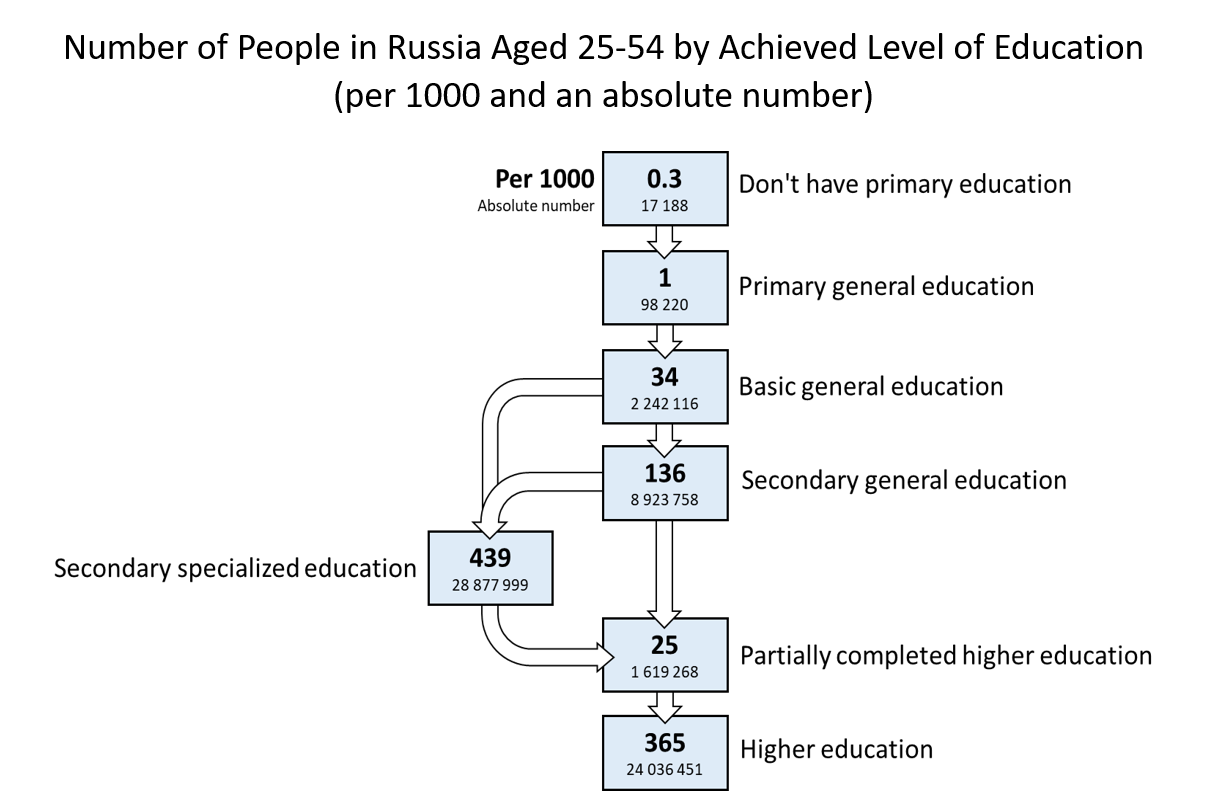
\includegraphics[width=5in]{graph_1c.png}
			% plot 1
		\end{minipage}
			\caption{Labor Force Distribution by Educational Level (Rosstat)}\label{fig:1.1a}
	\end{figure}
\end{center}


\vspace{-2em}


Figure \ref{fig:1.1a} indicates the educational attainment of the population segment 25 to 54 years, which is the age group for which Rosstat provides this information. Figure \ref{fig:1.1a}  shows less than 14\% of the labor force with a final attainment of secondary general education (academic High School) - the main choice is between vocational education (nearly 45\%) and university education (about 40\%). It is a well-known fact that on cognitive attainment at Grade 9, Russian students are already at par with OECD students (PISA scores are designed with an OECD mean of 500); what comes in later education levels and the labor market is the crucial issue for convergence with OECD on human capital wealth levels. 

A detailed analysis of the returns to education in the Russian Federation will provide insights into the stylized facts mentioned above. Together with other research being implemented by the World Bank and by researchers outside of the World Bank, the purpose of this analysis is to come up with a set of evidence based policy recommendations to enhance the human capital wealth of the Russian Federation. 

In this paper we report on an estimate of the private rate of return to investment in education in the Russian Federation. Human capital, or the stock of skills that is possessed by labor force, is pivotal in enabling countries and individuals to flourish in a multifaceted, increasingly comprehensive, interrelated, and rapidly changing society \parencite{Broecke2015}. The returns to investment in education have been a popular empirical analysis in research to study the relationship between schooling and earnings. Private returns can also explain the private demand for education. The literature suggests that each additional year of schooling produces a private (that is, individual) rate of return to schooling of about 8 to 10 percent a year \parencite{Psacharopoulos_Patrinos2018,Montenegro_Patrinos2014}. Globally, the returns to tertiary education are highest, followed by primary and then secondary schooling; this represents a significant reversal from many studies' prior results. Policy makers can learn much from Mincerian results; for instance, further expansion of university education appears to be very worthwhile for the individual, meaning that governments need to find ways to make financing more readily available, and that high rates of return are found through investment in girls' education.

\section{Literature}

In a worldwide perspective, the latest findings on returns to education can be condensed to the following \parencite{Psacharopoulos_Patrinos2018}: (1) overall, an amplified share of workers with tertiary education at the labor market has not reduced the magnitude of returns on the investment due to ``skill-biasedness'' of the technological progress boosting the demand for higher skills; (2) low- and middle-income regions are characterized by the largest returns except for outlying Middle East and North Africa having the lowest returns; (3) the private returns to education for women outstrip that of for men by roughly two percentage points; (4) private sector employees receive greater returns than those working in a public sector; (5) social returns to education are negatively associated with a country's level of economic development and education level; (6) on average, there is a growing trend in returns to higher education.

A separate, albeit scarce in terms of quantity, quality, and reliability, corpus of research focused on the Russian\slash USSR case. In the USSR during the period before education reforms the rates of return to schooling were strikingly low: 2-3\% for secondary and 5\% for higher education levels \parencite{Graeser1988}. Poor returns of human capital went in line with a planning economy offering free education, centralized allocation of labor force, and ideology of proletariat superiority; similar picture was observed in other ex-communist countries \parencite{Munich2005}.

However, an earlier attempt \dots \textcolor{red}{Boss, we did not understand this prompt} 

A group of scholars reported that during the transition period from a planned to market economy in Russia rates of returns to schooling rose sharply \parencite{Brainerd1998,Clark2003,Vernon2002}. The upsurge in wage premiums to education (especially university education) was asserted to be a pivotal factor that exacerbated wage dispersion: salaries of highly skilled and trained workers had gone up in absolute terms and compared to less-educated workers \parencite{Fleisher2005}. However, returns to schooling declined for those people who took advantage of higher education expansion in a post-communist Russia (1990-2005) in comparison to youths who obtained university degree in preceding periods \parencite{Kyui2016}. One researcher exploited data about the average education level at the end of a Soviet period as an instrument and inferred that the growth in the proportion of city dwellers with university degree was associated with a rise in the wages of  city residents \parencite{ Muravyev2008}.
Despite enhancements in premiums to tertiary (professional and higher) education in the Russian Federation at the beginning of the 2000s, the labor market was shown to be different from that of developed countries. Comparing Russia with France, the existence of a vertical education-occupation mismatch in Russia was demonstrated \parencite{Kyui2010}. A recent paper claims that horizontal education-job mismatch negatively impacts upon earnings of university graduates in all fields except for the low-paid ones \parencite{Rudakov2019}. Studies also suggest that education-job mismatch during studentship for individuals obtaining vocational education is "penalizing": combining studies with a job unrelated to a person's specialty entails a mismatch after his/her graduation \parencite{Dudyrev2018}.

Another research line ascertained that during the transition returns to education in Russia were not improving and remained among the most deficient in the world \parencite{Cheidvasser2007}. The contradiction with previous inferences and reasoning was explained by the omitted variable bias: past researchers did not account for regional covariates and rural area, thus ended up with overestimated return rates. It was highlighted that the excess of well-educated workers seemed to be the main underpinning factor of wage differentials in Russia after Soviet Union dissolution. Subsequently, Calvo et al. provided evidence on a reduction in skill premiums in Russia during the 2002 - 2012 period that was claimed to be one of the most relevant underlying forces explaining a deceleration in trends of widening wage inequality \parencite{Calvo2015}.
Belskaya et al. evaluated a large-scale college expansion in Russia after the breakdown of the Soviet Union \parencite{Belskaya2014}. Among the key conclusions is that as the number of university campuses grew, individuals with low returns to schooling grew as well. But for a marginal person, who switched into a treatment group as a result of new campuses opening, the total gains from attending a college are considerable and positive. Furthermore, the scholars found that students with higher returns are attracted more intensively by new campuses opened in constrained municipalities (small non-capital cities or those lacking higher education institutions before college expansion) in comparison to the unconstrained ones.
Like the global patterns, studies in Russia have shown that in the post-soviet decade workers, hired in firms controlled\slash owned by private organizations\slash individuals, retained a marked premium to education in contrast to workers employed in state companies. This is rooted in a greater flexibility of private firms, enabling to surmount restrictions caused by the rigidity of state wages, hence leading to larger returns to schooling \parencite{Clark2003}.
\cite{Borisov2007} was among the first who employed cohort analysis, using Mincerian wage equation for the Russian data, and found evidence favoring the existence of a powerful vintage effect (especially for men) at the labor market in Russia in the transition period: consecutive cohorts were paid more than the previous ones, keeping educational achievements constant; this phenomenon was entrenched in the specificity of a Soviet system, encouraging the pursuit of communist interests through extensive propaganda.
A source of heterogeneity in rates of returns to education in Russia hails from gender differences similar to the patterns ensured globally: women received greater returns to higher education than men (e.g., \cite{Cheidvasser2007}; \cite{Lukyanova2010}). 
By the end of the first decade of the 21st century some scholars detected positive changes concerning tertiary education in Russia (and other BRIC countries): payoff rates to university completion have generally magnified relative to the rates in lower levels of education and were higher than returns to secondary schooling \parencite{Carnoy2012}. This runs counter to the logic of capital theory, implying a decline in rank order of returns with education level, which should hold with a country's economic advancement. Private rate of returns even accounting for tuition cost in Russia is especially high in business\slash economics as a study field \parencite{Carnoy2012}. Additionally, rates of returns to vocational education were declared to be lower than payoffs to tertiary education \parencite{Borisov2007}. In a recent paper, \cite{Gimpelson2019} argued that the labor market in Russia might be at risk of over-education, which leads to a reduction in educational premiums.

 
\section{Data}

In this paper we use the Russian Longitudinal Monitoring Survey (RLMS) - the only representative Russian survey with a sizable panel component allowing for a dynamic analysis \parencite{Kozyreva2016}. The data are notable for their reliability, diversity, and applicability to a variety of research questions. The RLMS embraces information on people's income and expenditure structure, their material well-being, educational and occupational behavior, health state and nutrition, migration, etc.  RLMS sampling procedures have been thoroughly and extensively described elsewhere \parencite{Kozyreva2016}. The present research uses all 23 waves (1994 - 2018) that are available as of \today. Two years (1997 and 1999) are missing in the data because data was not collected in those years due to funding problems. The sub-sample selected for empirical investigation in this paper consists of working individuals aged 25-64 who are out of school and have positive labor market experience and income. 
\\

Table \ref{tab:1.1} shows descriptive statistics for the key variables under focus and sample sizes by years. The average years of experience is relatively stable over time, year of education slightly goes up with higher education level becoming increasingly popular in Russia.

\begin{table}[htbp!]
	\centering
	\caption{Descriptive Statistics, RLMS}
	\label{tab:1.1}	
	\resizebox{\textwidth}{!}{
		\begin{tabular}{lcccccccccc}
			\hline
			&  &  &  &  &  &  &  & \multicolumn{3}{c}{Education} \\ 
			&  & \multicolumn{2}{c}{Wage} & \multicolumn{2}{c}{Experience} & \multicolumn{2}{c}{Education years} & Secondary & Vocational & \multicolumn{1}{c}{Higher} \\ 
			Year  & N & Mean & SD & Mean & SD & Mean & SD & Percent & Percent & \multicolumn{1}{c}{Percent} \\ 
			\hline
			1994  & $3044$ & $\phantom{0}272761.9$ & $\phantom{0}347856.1$ & $\phantom{00000}21.4$ & $\phantom{000000}9.6$ & $\phantom{00000}12.7$ & $\phantom{000000}2.3$ & $\phantom{00000}22.3$ & $\phantom{00000}50.4$ & $\phantom{00000}27.3$ \\
			1995  & $2694$ & $\phantom{0}557844.7$ & $\phantom{0}621599.5$ & $\phantom{00000}21.7$ & $\phantom{000000}9.6$ & $\phantom{00000}12.7$ & $\phantom{000000}2.2$ & $\phantom{00000}22.3$ & $\phantom{00000}47.8$ & $\phantom{00000}29.8$ \\
			1996  & $2282$ & $\phantom{0}817936.7$ & $1004035.7$ & $\phantom{00000}21.6$ & $\phantom{000000}9.6$ & $\phantom{00000}12.8$ & $\phantom{000000}2.2$ & $\phantom{00000}19.7$ & $\phantom{00000}48.6$ & $\phantom{00000}31.7$ \\
			1998  & $3102$ & $\phantom{0000}906.3$ & $\phantom{0000}950.7$ & $\phantom{00000}22.3$ & $\phantom{000000}9.6$ & $\phantom{00000}12.7$ & $\phantom{000000}2.2$ & $\phantom{00000}19.8$ & $\phantom{00000}52.0$ & $\phantom{00000}28.2$ \\
			2000  & $3215$ & $\phantom{000}1821.3$ & $\phantom{000}2570.5$ & $\phantom{00000}22.3$ & $\phantom{00000}10.0$ & $\phantom{00000}12.7$ & $\phantom{000000}2.2$ & $\phantom{00000}20.3$ & $\phantom{00000}51.3$ & $\phantom{00000}28.4$ \\
			2001  & $3605$ & $\phantom{000}2681.0$ & $\phantom{000}2849.6$ & $\phantom{00000}22.0$ & $\phantom{000000}9.8$ & $\phantom{00000}12.8$ & $\phantom{000000}2.2$ & $\phantom{00000}19.8$ & $\phantom{00000}49.3$ & $\phantom{00000}30.9$ \\
			2002  & $3803$ & $\phantom{000}3612.8$ & $\phantom{000}4316.0$ & $\phantom{00000}22.0$ & $\phantom{000000}9.9$ & $\phantom{00000}12.8$ & $\phantom{000000}2.1$ & $\phantom{00000}19.3$ & $\phantom{00000}49.9$ & $\phantom{00000}30.8$ \\
			2003  & $3858$ & $\phantom{000}4378.6$ & $\phantom{000}4014.0$ & $\phantom{00000}22.2$ & $\phantom{00000}10.1$ & $\phantom{00000}12.8$ & $\phantom{000000}2.2$ & $\phantom{00000}19.1$ & $\phantom{00000}49.4$ & $\phantom{00000}31.5$ \\
			2004  & $3968$ & $\phantom{000}5379.0$ & $\phantom{000}4918.5$ & $\phantom{00000}22.0$ & $\phantom{00000}10.2$ & $\phantom{00000}12.8$ & $\phantom{000000}2.2$ & $\phantom{00000}18.4$ & $\phantom{00000}50.3$ & $\phantom{00000}31.2$ \\
			2005  & $3913$ & $\phantom{000}6637.9$ & $\phantom{000}5716.1$ & $\phantom{00000}22.1$ & $\phantom{00000}10.4$ & $\phantom{00000}12.8$ & $\phantom{000000}2.2$ & $\phantom{00000}18.4$ & $\phantom{00000}49.6$ & $\phantom{00000}32.0$ \\
			2006  & $4804$ & $\phantom{000}8089.9$ & $\phantom{000}6563.9$ & $\phantom{00000}22.2$ & $\phantom{00000}10.4$ & $\phantom{00000}12.8$ & $\phantom{000000}2.2$ & $\phantom{00000}18.0$ & $\phantom{00000}50.9$ & $\phantom{00000}31.1$ \\
			2007  & $4726$ & $\phantom{000}9662.5$ & $\phantom{000}7124.7$ & $\phantom{00000}22.5$ & $\phantom{00000}10.6$ & $\phantom{00000}12.8$ & $\phantom{000000}2.2$ & $\phantom{00000}18.5$ & $\phantom{00000}50.2$ & $\phantom{00000}31.3$ \\
			2008  & $4827$ & $\phantom{00}12826.3$ & $\phantom{00}10784.5$ & $\phantom{00000}22.6$ & $\phantom{00000}10.8$ & $\phantom{00000}12.9$ & $\phantom{000000}2.3$ & $\phantom{00000}17.9$ & $\phantom{00000}47.8$ & $\phantom{00000}34.3$ \\
			2009  & $4804$ & $\phantom{00}13363.1$ & $\phantom{00}10411.4$ & $\phantom{00000}22.5$ & $\phantom{00000}11.0$ & $\phantom{00000}12.9$ & $\phantom{000000}2.3$ & $\phantom{00000}16.6$ & $\phantom{00000}47.9$ & $\phantom{00000}35.5$ \\
			2010  & $7326$ & $\phantom{00}14769.9$ & $\phantom{00}12587.1$ & $\phantom{00000}22.6$ & $\phantom{00000}11.1$ & $\phantom{00000}13.0$ & $\phantom{000000}2.3$ & $\phantom{00000}16.9$ & $\phantom{00000}48.1$ & $\phantom{00000}34.9$ \\
			2011  & $7167$ & $\phantom{00}16226.8$ & $\phantom{00}12855.5$ & $\phantom{00000}22.5$ & $\phantom{00000}11.1$ & $\phantom{00000}13.0$ & $\phantom{000000}2.3$ & $\phantom{00000}18.0$ & $\phantom{00000}46.9$ & $\phantom{00000}35.1$ \\
			2012  & $7428$ & $\phantom{00}18880.7$ & $\phantom{00}15119.0$ & $\phantom{00000}22.5$ & $\phantom{00000}11.2$ & $\phantom{00000}13.0$ & $\phantom{000000}2.4$ & $\phantom{00000}18.2$ & $\phantom{00000}45.9$ & $\phantom{00000}35.9$ \\
			2013  & $7327$ & $\phantom{00}20601.4$ & $\phantom{00}16411.5$ & $\phantom{00000}22.5$ & $\phantom{00000}11.2$ & $\phantom{00000}13.1$ & $\phantom{000000}2.3$ & $\phantom{00000}17.0$ & $\phantom{00000}46.7$ & $\phantom{00000}36.3$ \\
			2014  & $6148$ & $\phantom{00}22772.6$ & $\phantom{00}17288.4$ & $\phantom{00000}22.3$ & $\phantom{00000}11.1$ & $\phantom{00000}13.1$ & $\phantom{000000}2.3$ & $\phantom{00000}16.5$ & $\phantom{00000}45.8$ & $\phantom{00000}37.7$ \\
			2015  & $6231$ & $\phantom{00}23570.7$ & $\phantom{00}16996.4$ & $\phantom{00000}22.2$ & $\phantom{00000}11.2$ & $\phantom{00000}13.2$ & $\phantom{000000}2.3$ & $\phantom{00000}15.2$ & $\phantom{00000}44.4$ & $\phantom{00000}40.4$ \\
			2016  & $6297$ & $\phantom{00}24951.1$ & $\phantom{00}18640.7$ & $\phantom{00000}22.3$ & $\phantom{00000}11.1$ & $\phantom{00000}13.3$ & $\phantom{000000}2.3$ & $\phantom{00000}14.7$ & $\phantom{00000}43.6$ & $\phantom{00000}41.8$ \\
			2017  & $6359$ & $\phantom{00}26254.1$ & $\phantom{00}19555.4$ & $\phantom{00000}22.4$ & $\phantom{00000}11.0$ & $\phantom{00000}13.3$ & $\phantom{000000}2.3$ & $\phantom{00000}14.0$ & $\phantom{00000}45.0$ & $\phantom{00000}40.9$ \\
			2018  & $6121$ & $\phantom{00}28081.0$ & $\phantom{00}19705.8$ & $\phantom{00000}22.5$ & $\phantom{00000}10.8$ & $\phantom{00000}13.3$ & $\phantom{000000}2.3$ & $\phantom{00000}13.8$ & $\phantom{00000}45.0$ & $\phantom{00000}41.2$ \\
			\hline 
		\end{tabular}
	}
\end{table}

\section{Methodology}

The Mincer equation-arguably the most widely used in empirical work-can be used to explain a host of economic, and even non-economic, phenomena. One such application involves explaining (and estimating) employment earnings as a function of schooling and labor market experience. The Mincer equation provides estimates of the average monetary returns of one additional year of education. This information is important for policy makers who must decide on education spending, prioritization of schooling levels, and education financing programs such as student loans \parencite{Patrinos2016}. In that respect, the Mincer equation is the most used econometric framework for estimating the rate of return in education.


The empirical analysis in this paper presents results for the general working population of the Russian Federation aged 25-64. We use a basic Mincerian specification shown in equation \eqref{eq:1.1}: 


\begin{flalign}\label{eq:1.1} 
Log(Wage) = b_0 + b_1\cdot Educ + b_2\cdot Exp + b_3\cdot Exp^2 + \epsilon
\end{flalign}


\noindent
where $Log(Wage)$ is a logarithm of monthly wage, $Educ$ stands for the years of education or highest attained level of education, $Exp$ and $Exp^2$ reflect the years of working experience and its quadratic term respectively, $b_0$ is an intercept, $b_1 ... b_n$ are the respective slope estimates, $\epsilon$ refers to a normally distributed error term.

%\subsection{Measures}

\textbf{Dependent variable}

For the dependent variable, we used the logarithm of an average monthly wage within the past year on a person's primary job (variable $J13.2$ in the RLMS dataset). If a person had an additional job, the maximum wage value among the two (variables $J13.2$ and $J40$) was selected for the analysis. In the waves from 1994 to 1996, the question mentioned above was absent; for those waves, we exploited a variable about the average amount of money earned by a respondent within the past 30 days (variable $J10$) as a reasonable approximation.

\textbf{Independent variables}

The present research uses both metric (measured in years) and categorical education variables. The metric version was created by assigning the average expected number of years corresponding to each attained education level. For the categorical version (EDUC), we distinguished three categories: \textit{(1) secondary, (2) vocational, and (3) higher}. Incomplete levels were incorporated into the respective upper categories (e.g., incomplete higher - into higher). We are interested in exploring returns to education in general, and vocational and higher education. Estimations of premiums to primary and secondary schooling levels are technically unreachable to us since the number of adults without primary education, and the number of adults with only primary level is minuscule in the general population. The experience variable was calculated as a difference between current age and years of education minus $6$. Regression \eqref{eq:1.1} was estimated separately for each year for the entire sample and separately for males and females. The Appendix presents the results for each year. 


We are particularly interested in the returns to specific levels of education, estimated through a series of dummy variables. Using Secondary Education completed as the base or omitted dummy for purpose of interpretation, we use dummies for Vocational Education and for Higher Education. The specification is presented in equation \eqref{eq:1.2}: 

\begin{flalign}\label{eq:1.2} 
Log(Wage) = a_0 + a_1\cdot D_{Voc} + a_2\cdot D_{Higher} + a_3\cdot Exp + a_4\cdot Exp^2 + a_5\cdot Gender + \epsilon
\end{flalign}



\section{Results}

Figure \ref{fig:5.1} demonstrates earnings ratio by educational level (secondary education is equal to 100\%) for 1998, 2006, and 2018. The graph depicts a pronounced gap in the wages of people with secondary or vocational education compared to those with university level especially in earlier years in Russia.

\vspace{-0.2in}
\begin{center}
	\begin{figure}[htbp!]
\begin{minipage}[b]{1\linewidth}
			\centering
			\hspace*{-0.6in}
			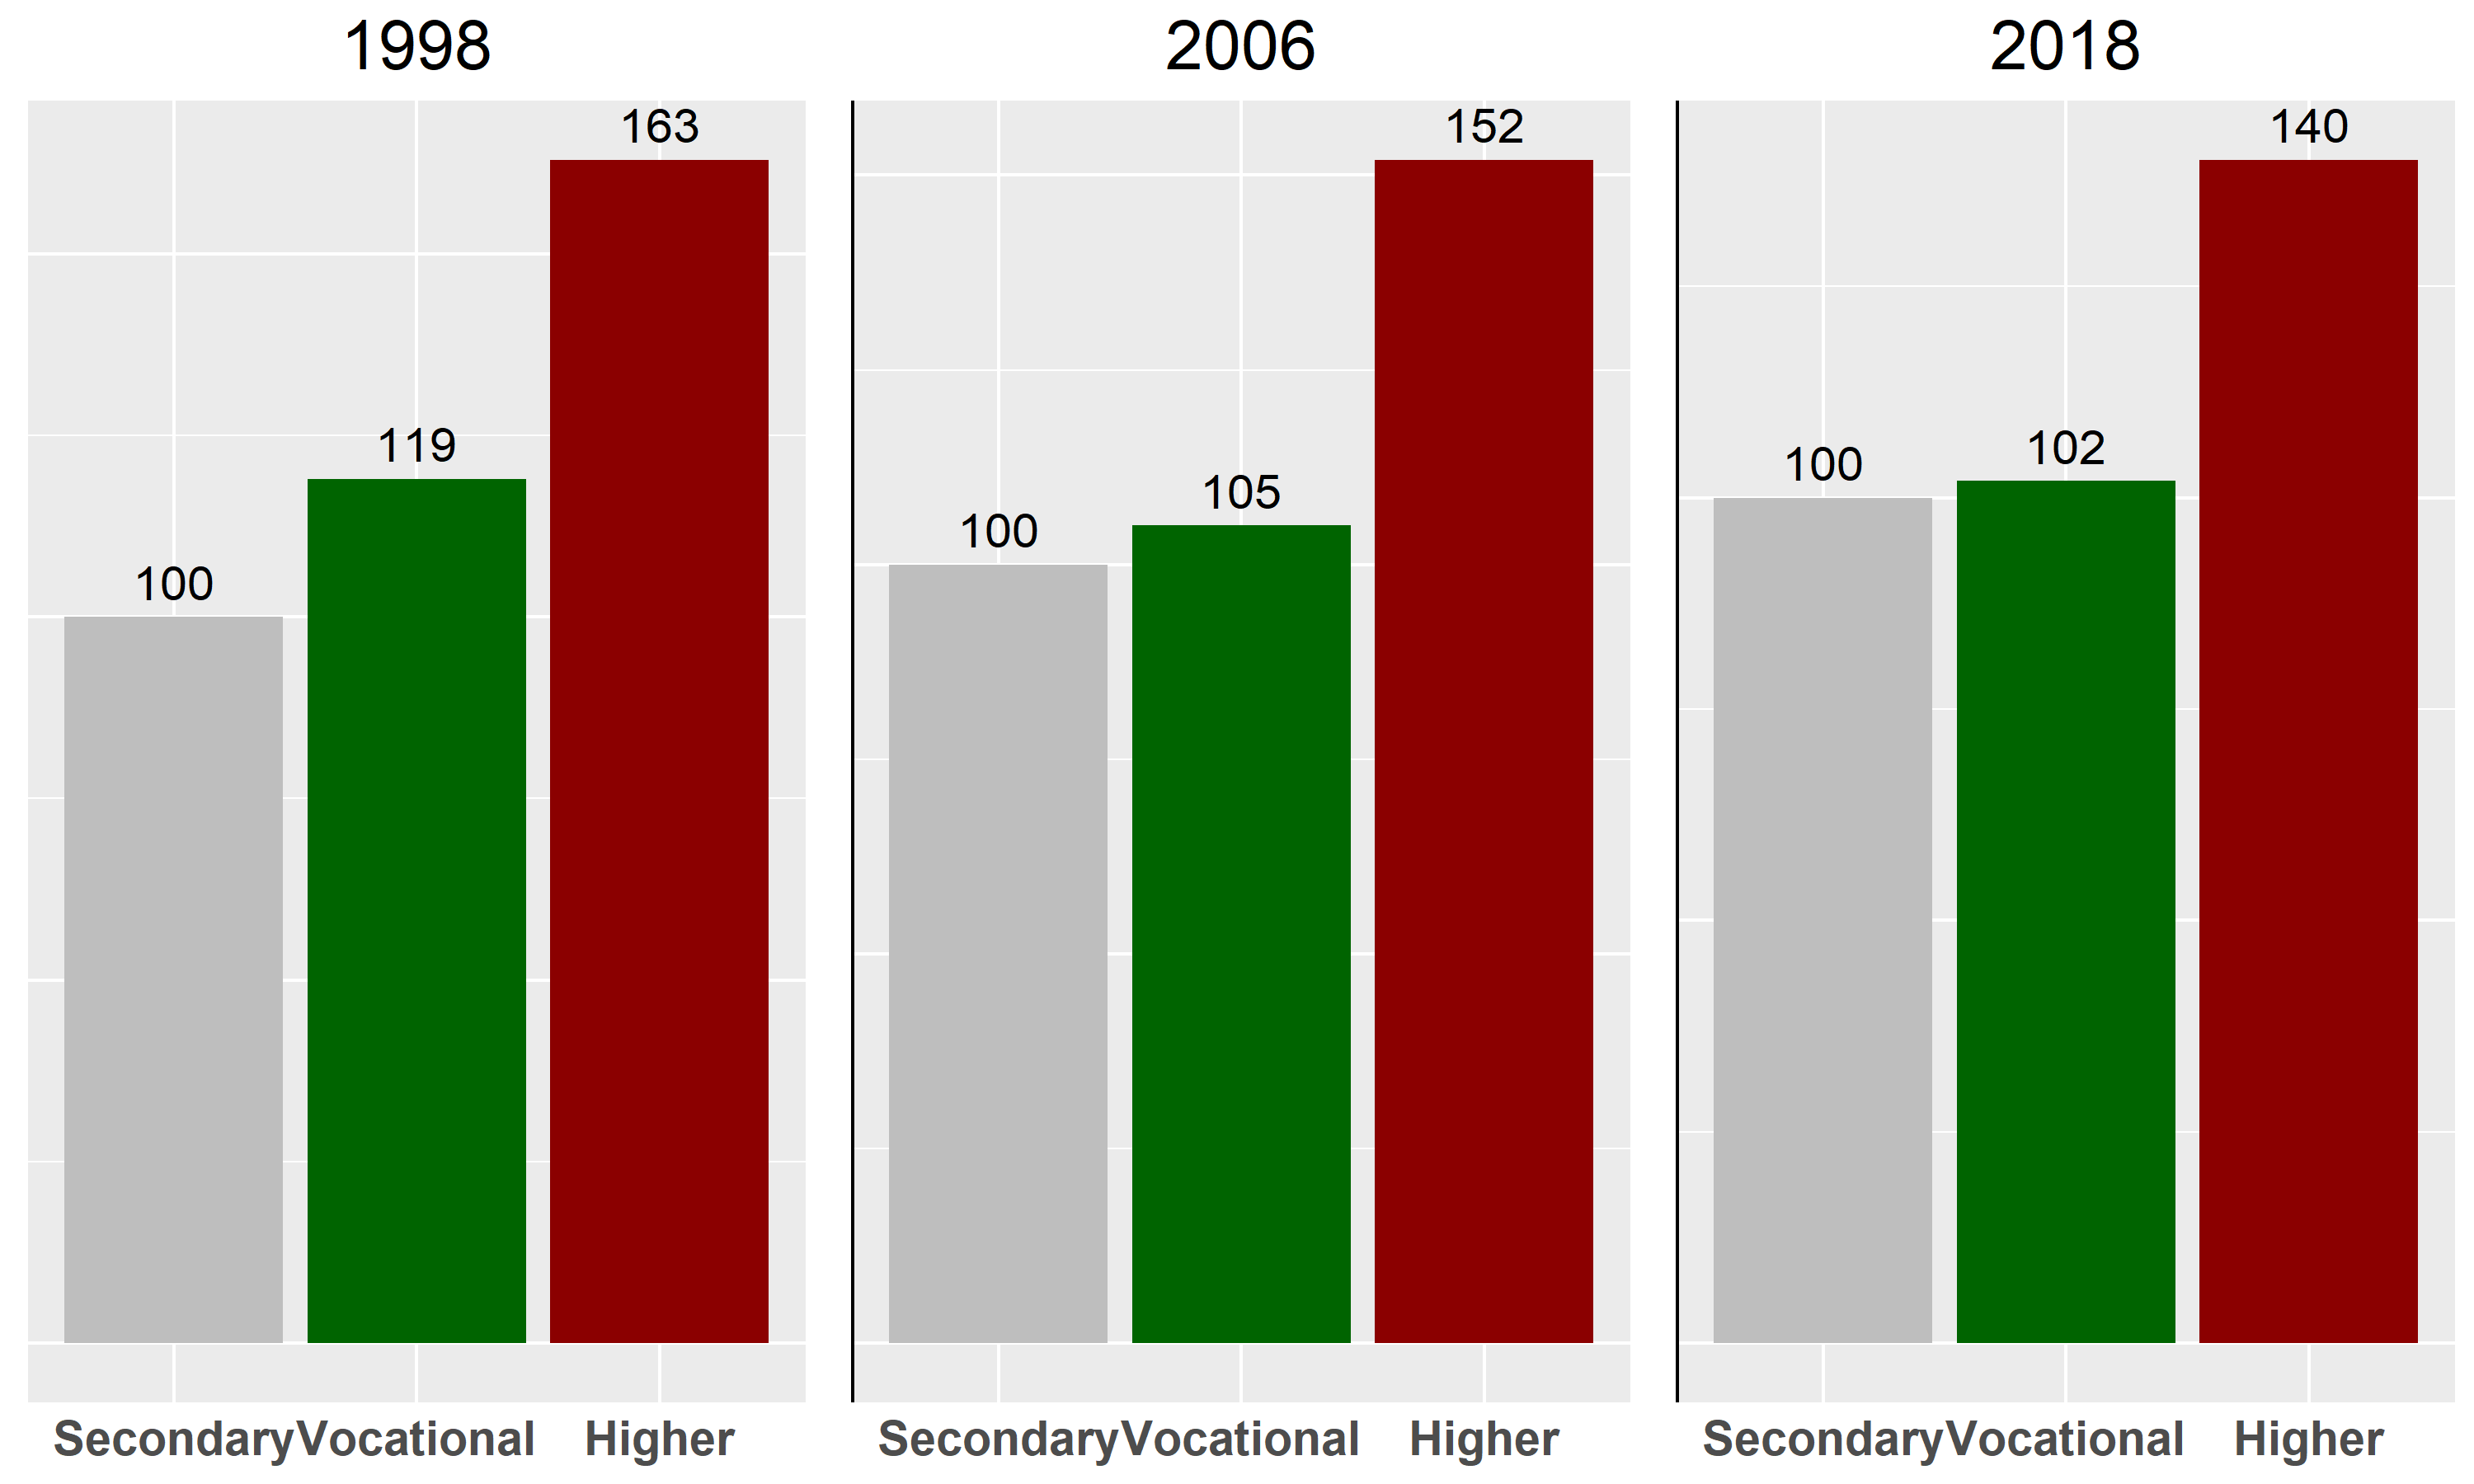
\includegraphics[width=5in]{earnings_ratio.png}
			% plot 1
		\end{minipage}
			\caption{Earnings Ratio by Educational Level (Secondary Education = 100\%)}\label{fig:5.1}
	\end{figure}
\end{center}

\vspace{-0.2in}

\begin{center}
	\begin{figure}[htbp!]
\begin{minipage}[b]{1\linewidth}
			\centering
			\hspace*{-0.3in}
			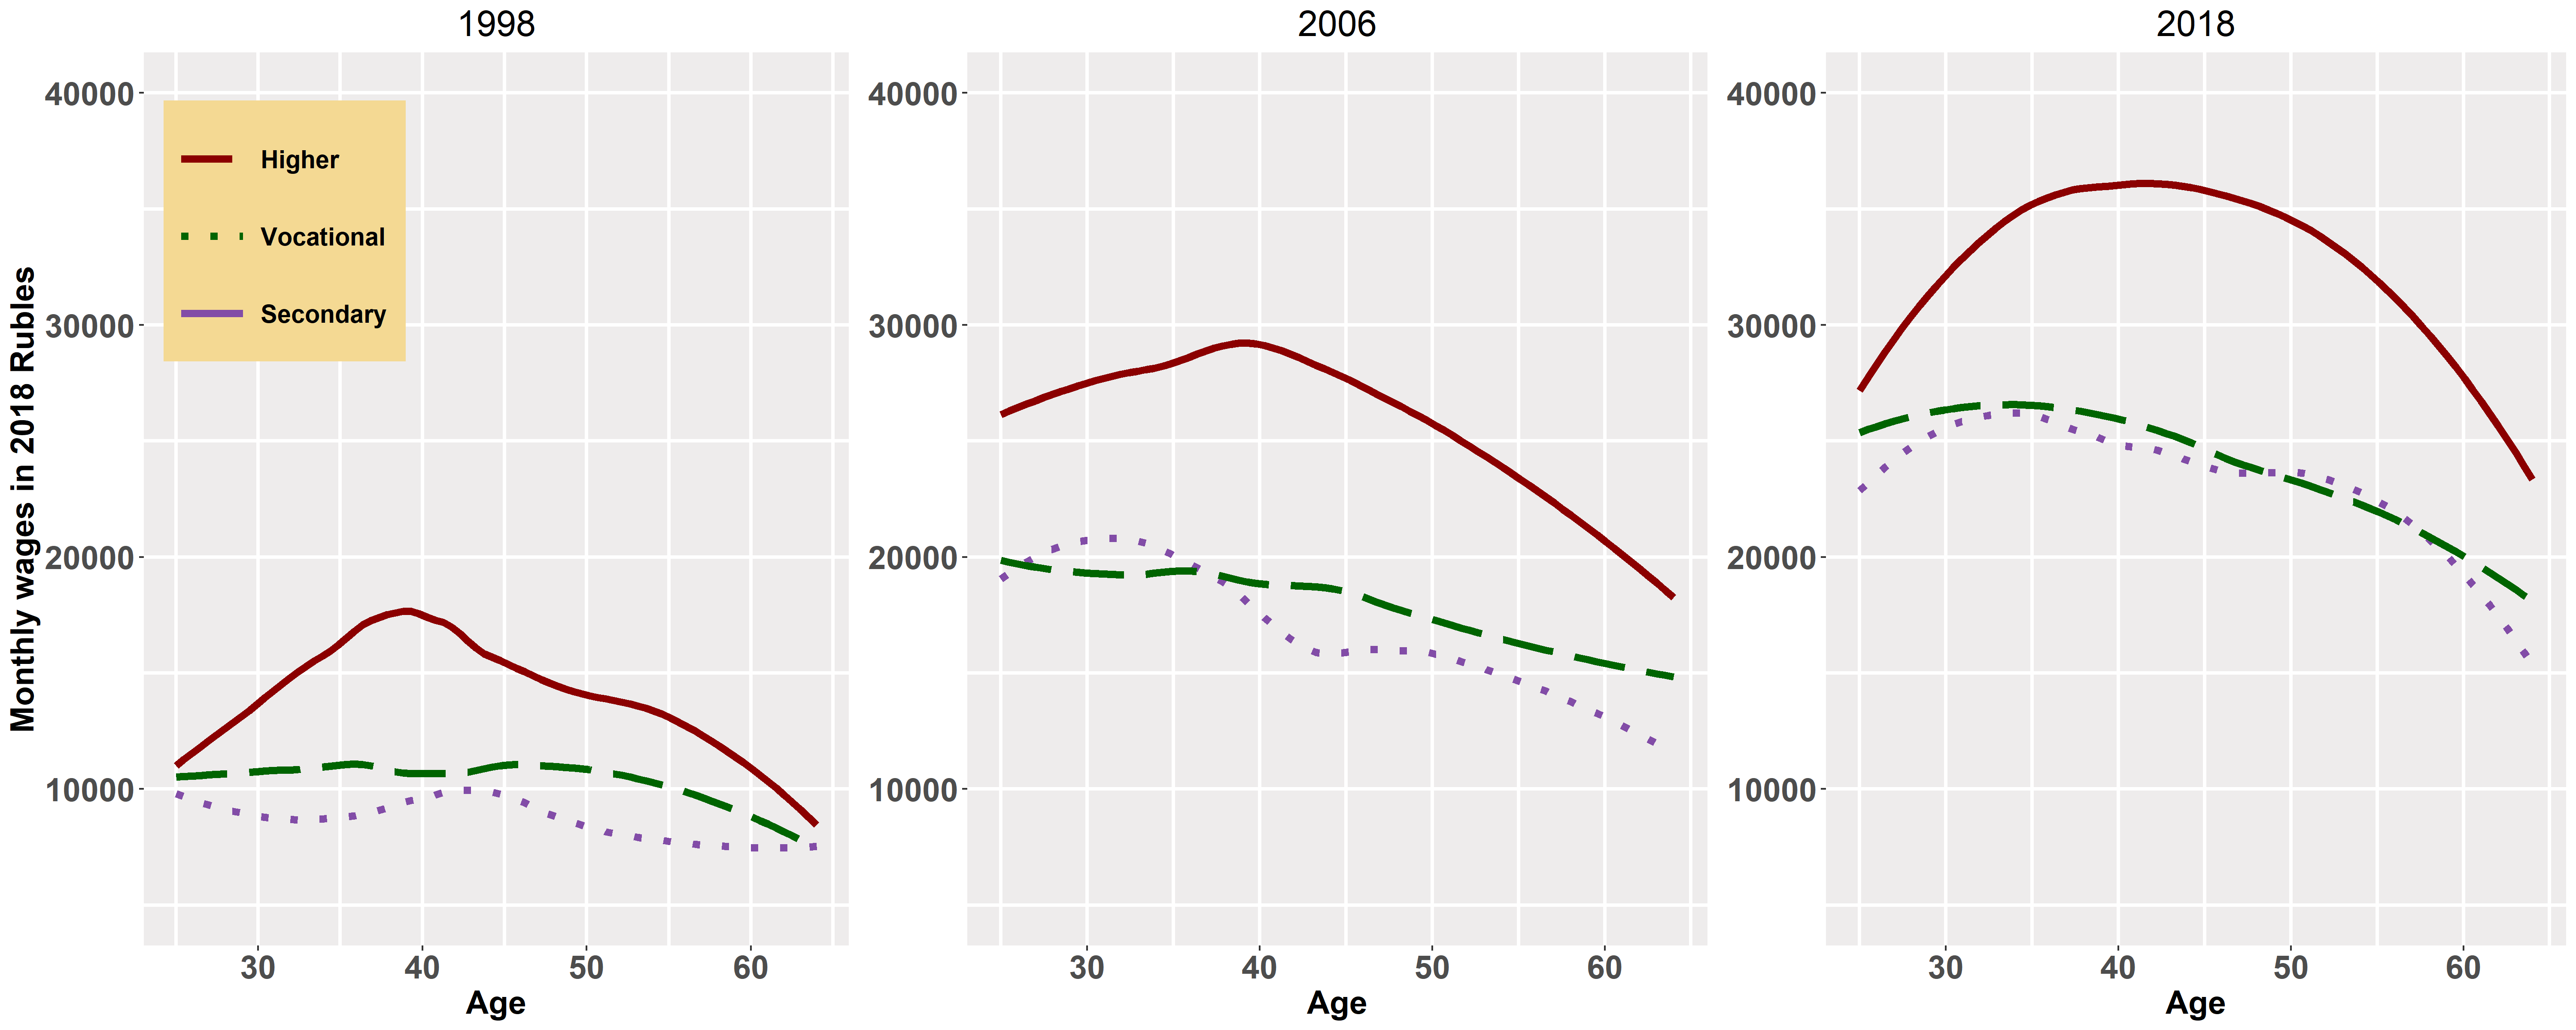
\includegraphics[width=6in]{earnings_by_level.png}
			% plot 1
		\end{minipage}
			\caption{Age-earning Profiles by Level of Education}\label{fig:5.2}
	\end{figure}
\end{center}

\vspace{-0.2in}

Figure \ref{fig:5.2} displays age-earning profiles in Russia by education level. There is a clear concave pattern for higher level, whereas for secondary and vocational levels, the association between wages and age is almost flat or descending.

Figure \ref{fig:1.2} summarizes the results, showing rates of overall and gender-wise returns to education in Russia for the period 1994-2018: the percentage increment in a person's earnings due to one additional year of schooling. Overall, one can notice a moderate curved growth in returns to education in Russia, achieving its peak in the early 2000s (returns of 9.8\%), which is followed by a downward pattern (returns of 5.6\% by 2018). The values of returns to schooling in recent years in Russia seem to lag far behind the global average of 9.5\% \parencite{Psacharopoulos_Patrinos2018}. Education payoffs for women are higher than those of men, but the difference appears to have narrowed in recent years.

Figure \ref{fig:1.3}, panel (a) displays rates of returns to Higher and Vocational education (as compared to Secondary education) in Russia for the period 1994-2018. The results suggest that on average wage premiums to university education in Russia are roughly 3-5 times greater than to vocational schooling. The observed trend for premiums to both Vocational and Higher education levels is similar to the trend for education in general with the following peaks: 18\% per year for Higher education and 6\% per year for Vocational education compared to the average earnings of workers with a Secondary education. The interesting pattern to note from panel \ref{fig:1.3a} is the apparent co-movement of vocational education and higher education - the higher education smoothing curve turns a bit more sharply than the one for vocational education, but their movement is matching, even at second-order levels of smoothness. Further, even though higher education premium remains much above the premium for vocational education, there is a perceptible narrowing of the difference in recent years. Panel \ref{fig:1.3b}, which is drawn from a presentation made by Marina Telezhkina at the WB-HSE Summer School on the Economics of Education in July 2019, shows the interesting pattern of higher education enrollment rates for the population of 17-25 year olds. Panel \ref{fig:1.3b} shows the downturn in returns reflected in enrollments, with the peak in enrollments coming about 10 years later. 

\begin{figure}[htbp!]
\caption{\textbf{Rates of Returns to Higher and Vocational Education in Russia, RLMS 1994-2018}}\label{fig:1.3}
         \centering
         \begin{subfigure}[b]{0.5\textwidth}
                 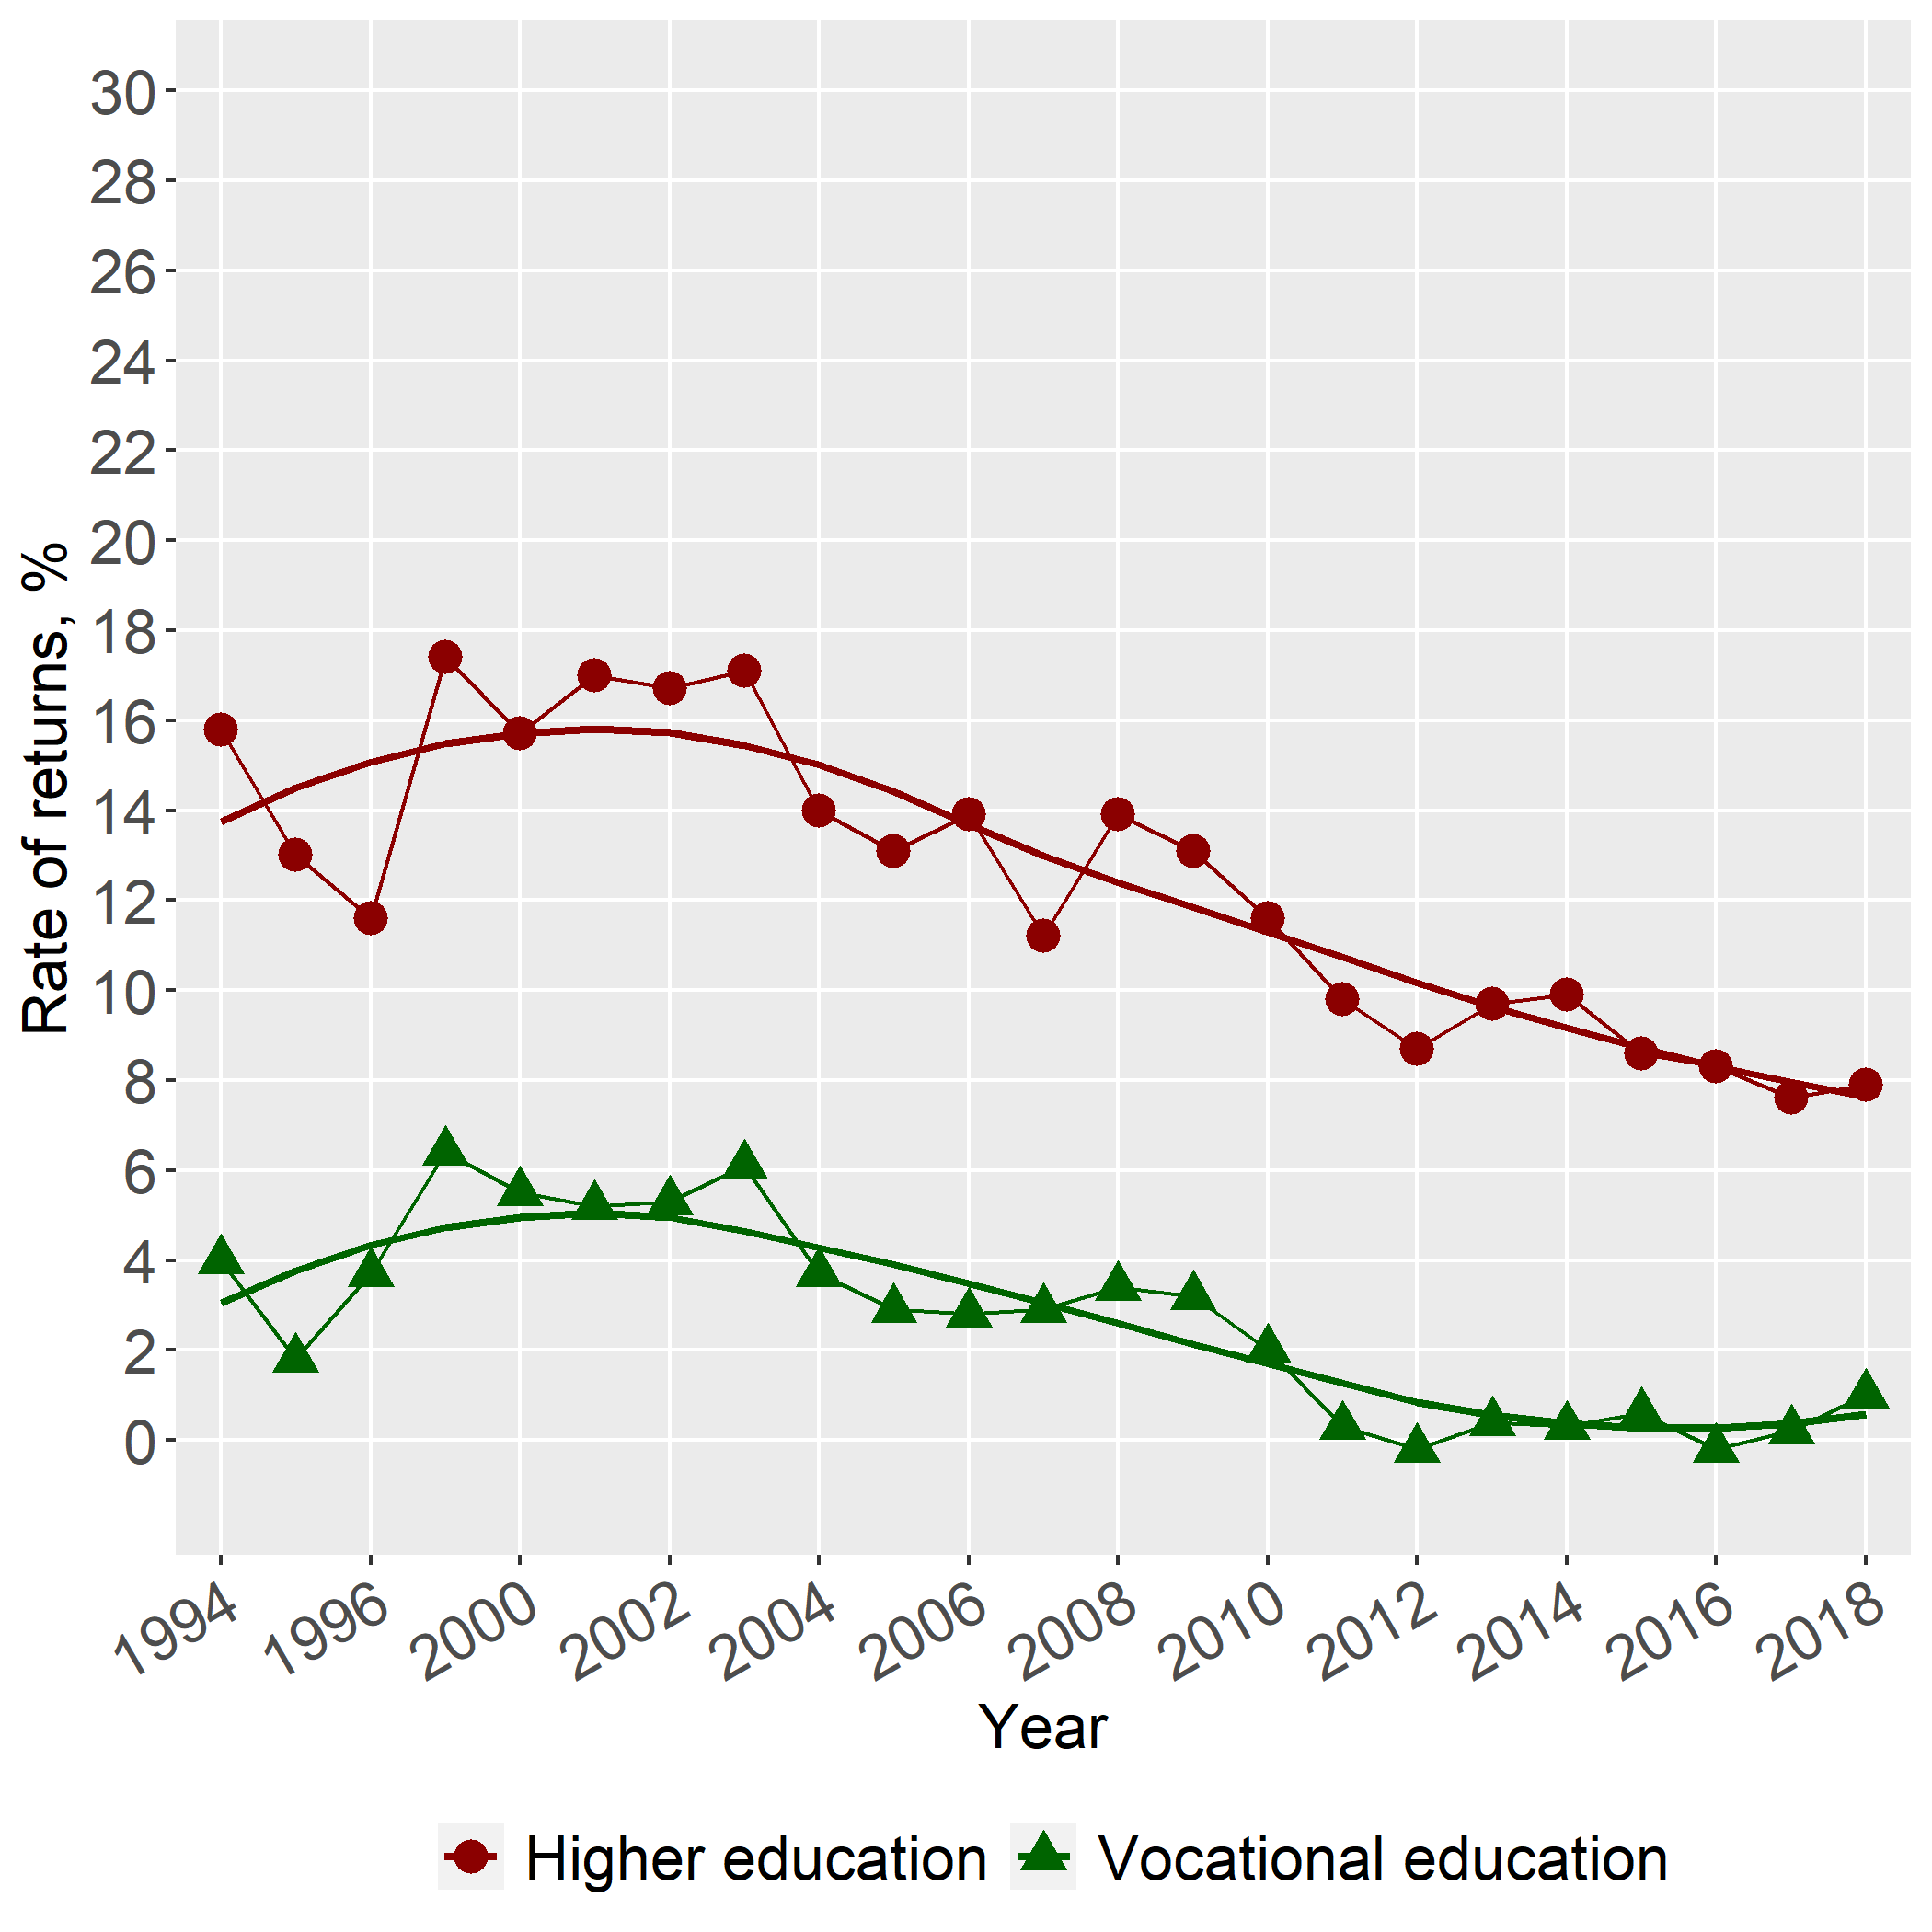
\includegraphics[width=\textwidth]{re_HE_all.png}
                 \caption{Rates of Return}
                 \label{fig:1.3a}
         \end{subfigure}%
         ~ %add desired spacing between images, e. g. ~, \quad, \qquad, \hfill etc.
           %(or a blank line to force the subfigure onto a new line)
         \begin{subfigure}[b]{0.5\textwidth}
                 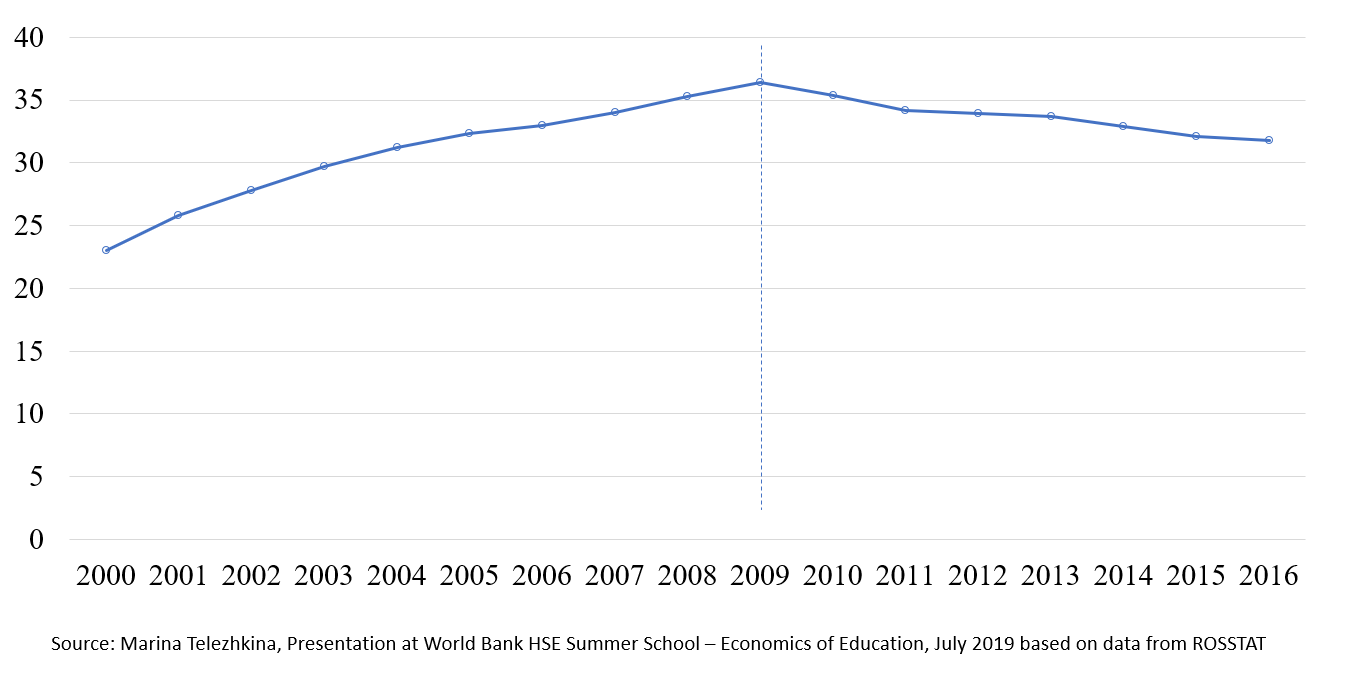
\includegraphics[width=\textwidth]{telezhkina.png}
                 \caption{Enrollment in Higher Education}
                 \label{fig:1.3b}
         \end{subfigure}
     \end{figure}


\begin{figure}[htbp!]
 \centering
 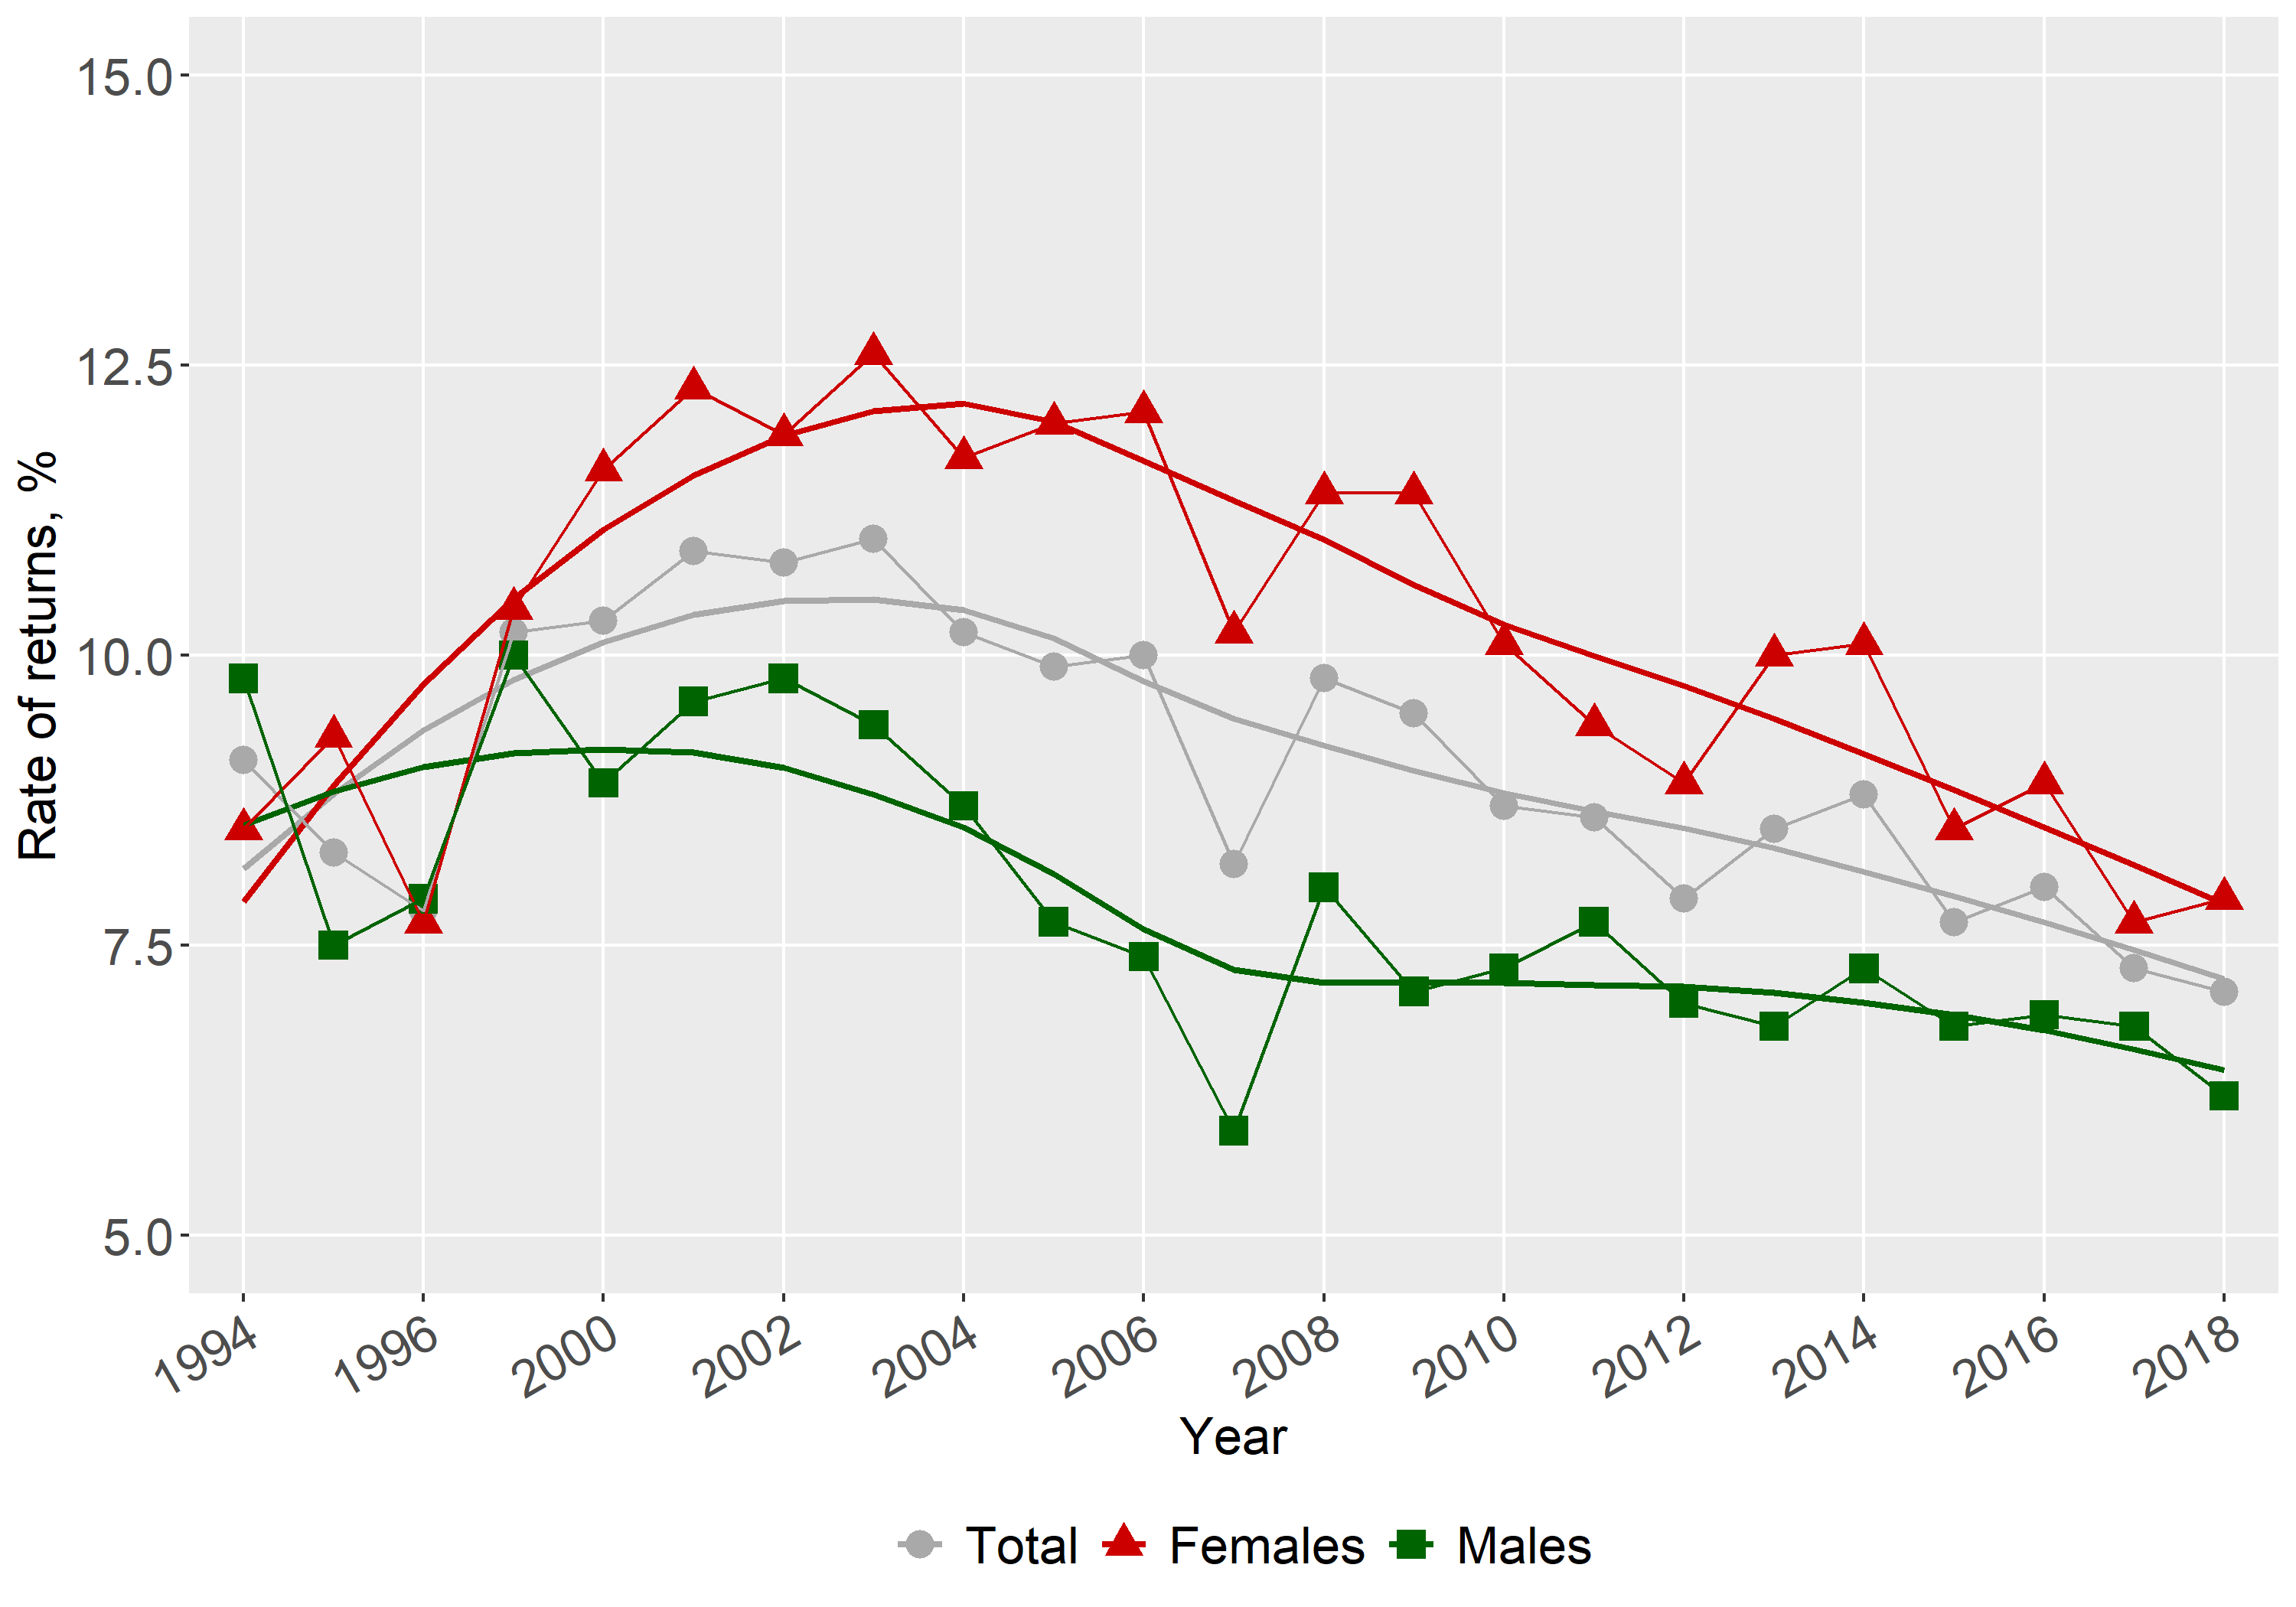
\includegraphics[width=\textwidth, height=275pt]{re_edu.png}
 \caption{Rates of Returns to Education in Russia, RLMS 1994-2018}\label{fig:1.2}
\end{figure}

\begin{figure}[htbp!]
  \begin{minipage}[b]{.5\linewidth}
     \centering
     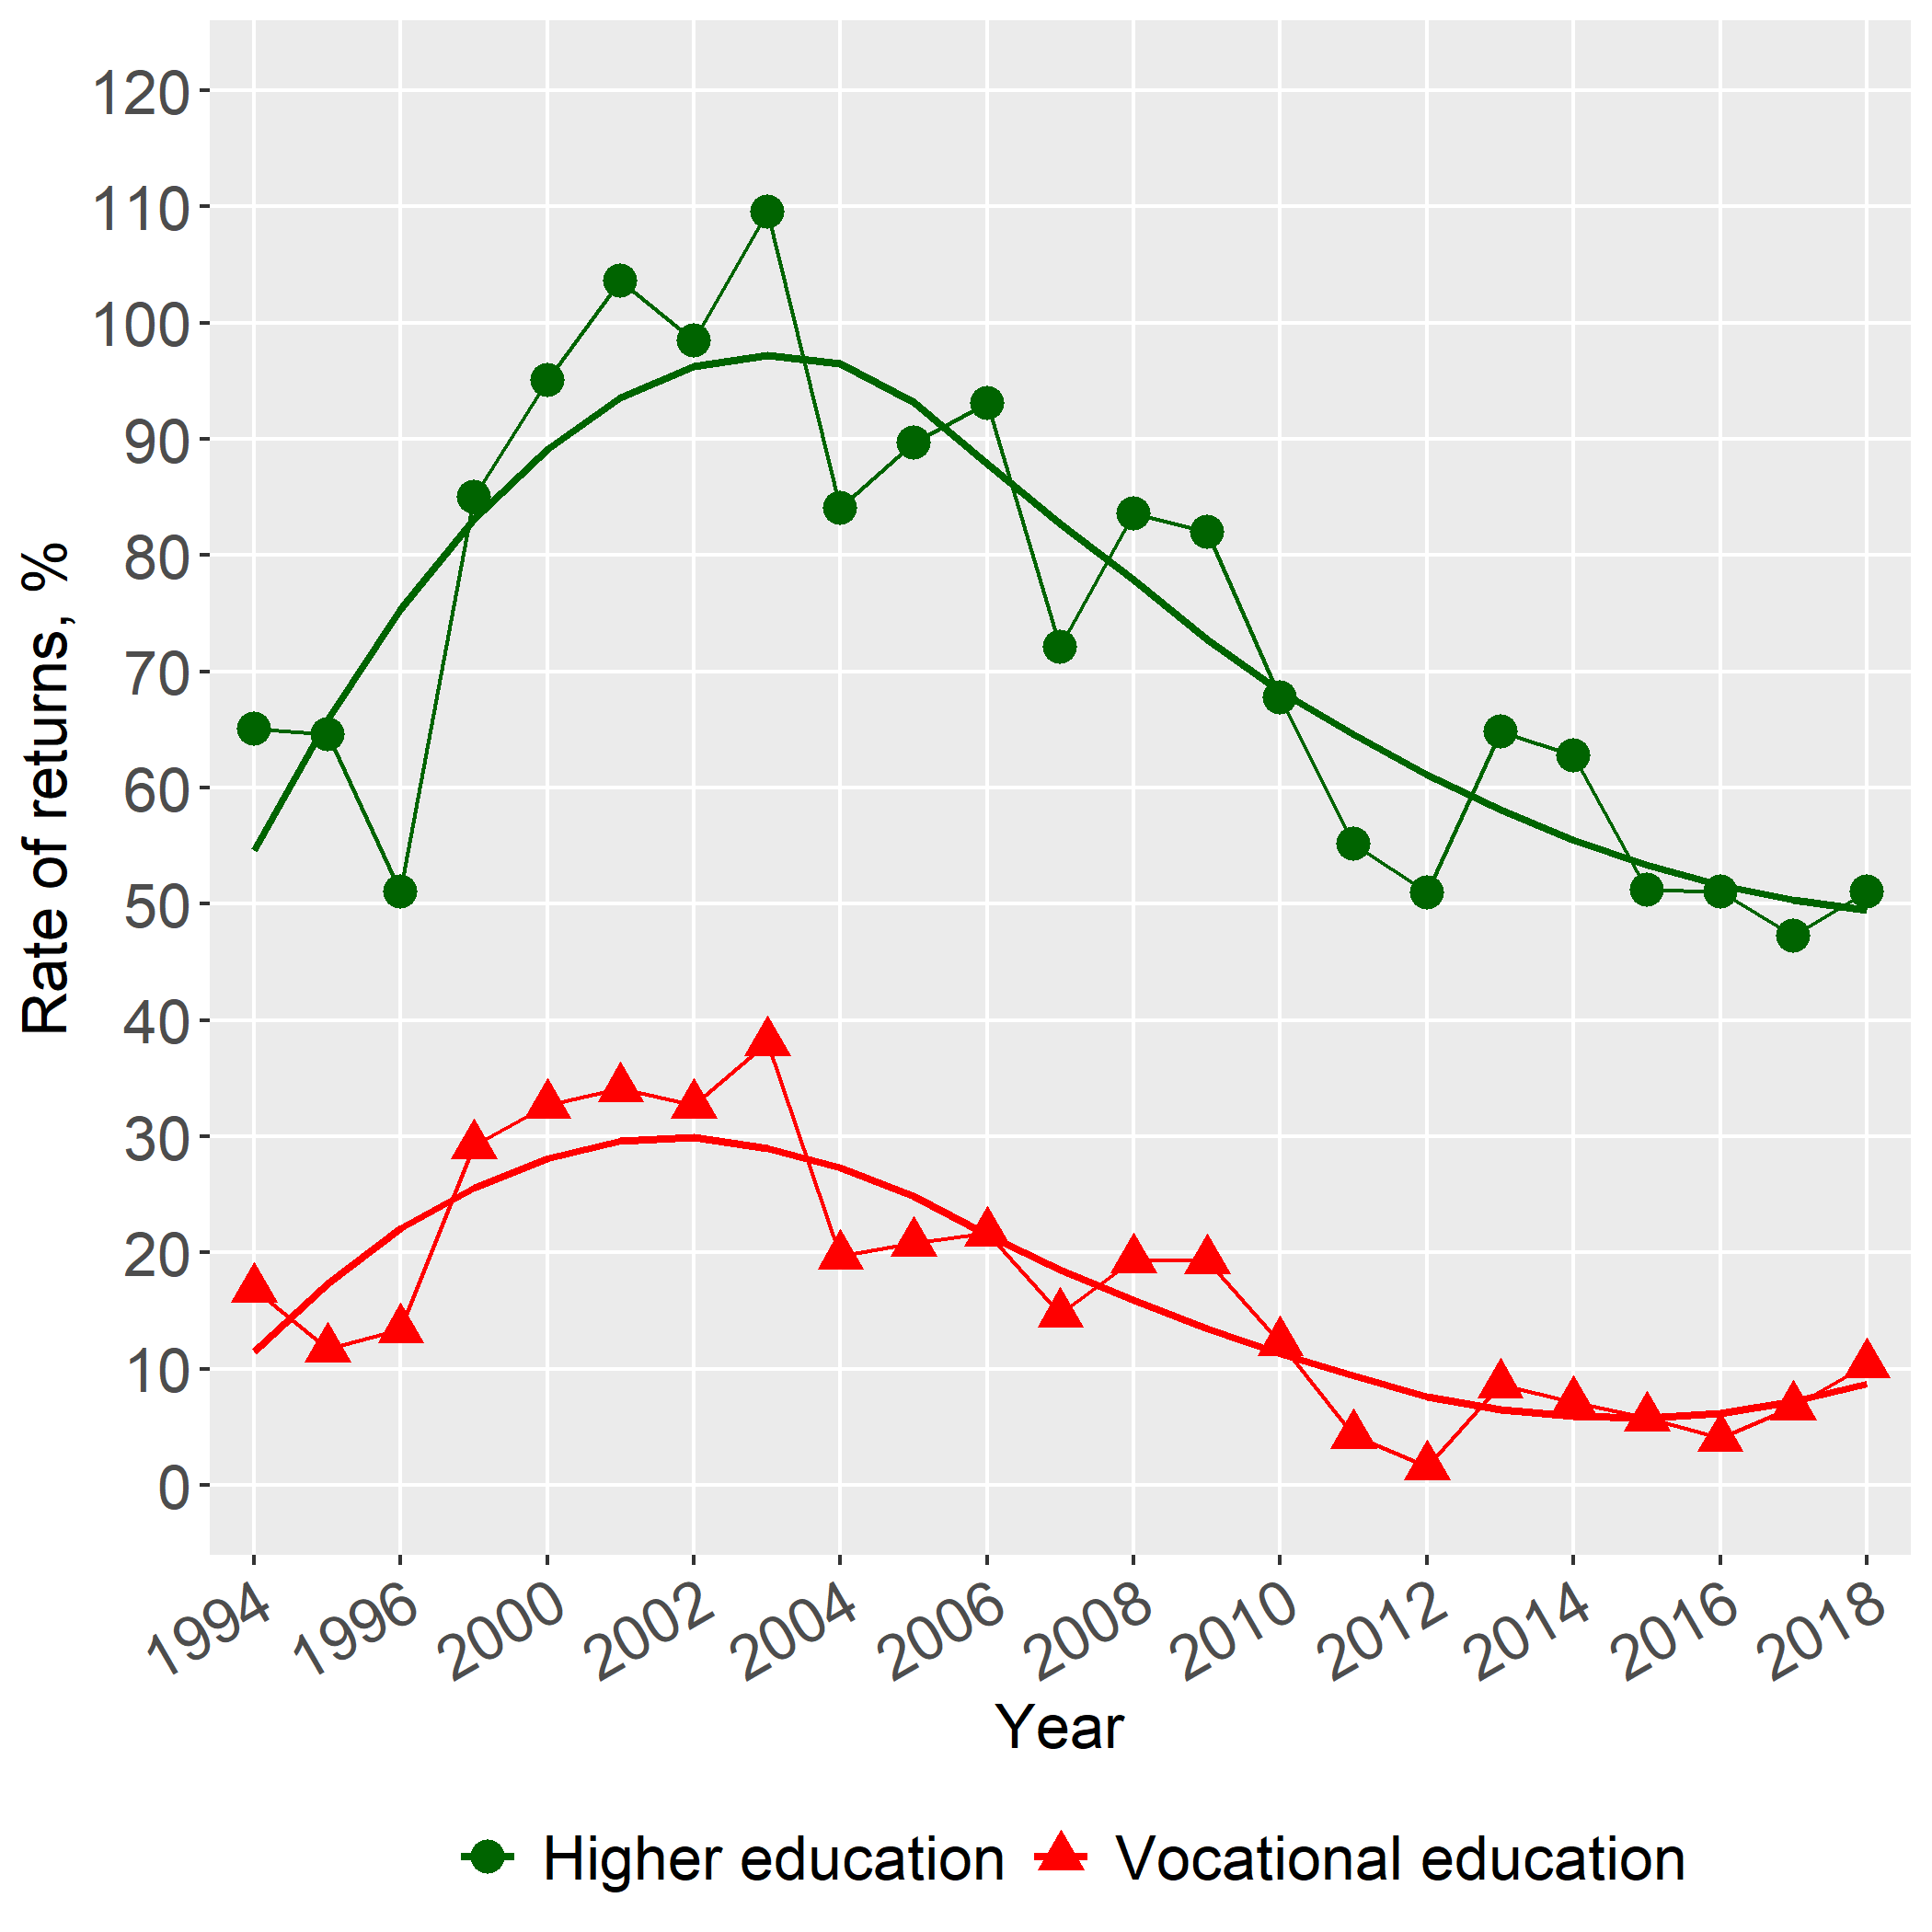
\includegraphics[width=\textwidth]{re_HE_f.png}
     % plot 1
     \subcaption{Females}\label{fig:1.4a}
  \end{minipage}
  \hfill
  \begin{minipage}[b]{.5\linewidth}
     \centering
     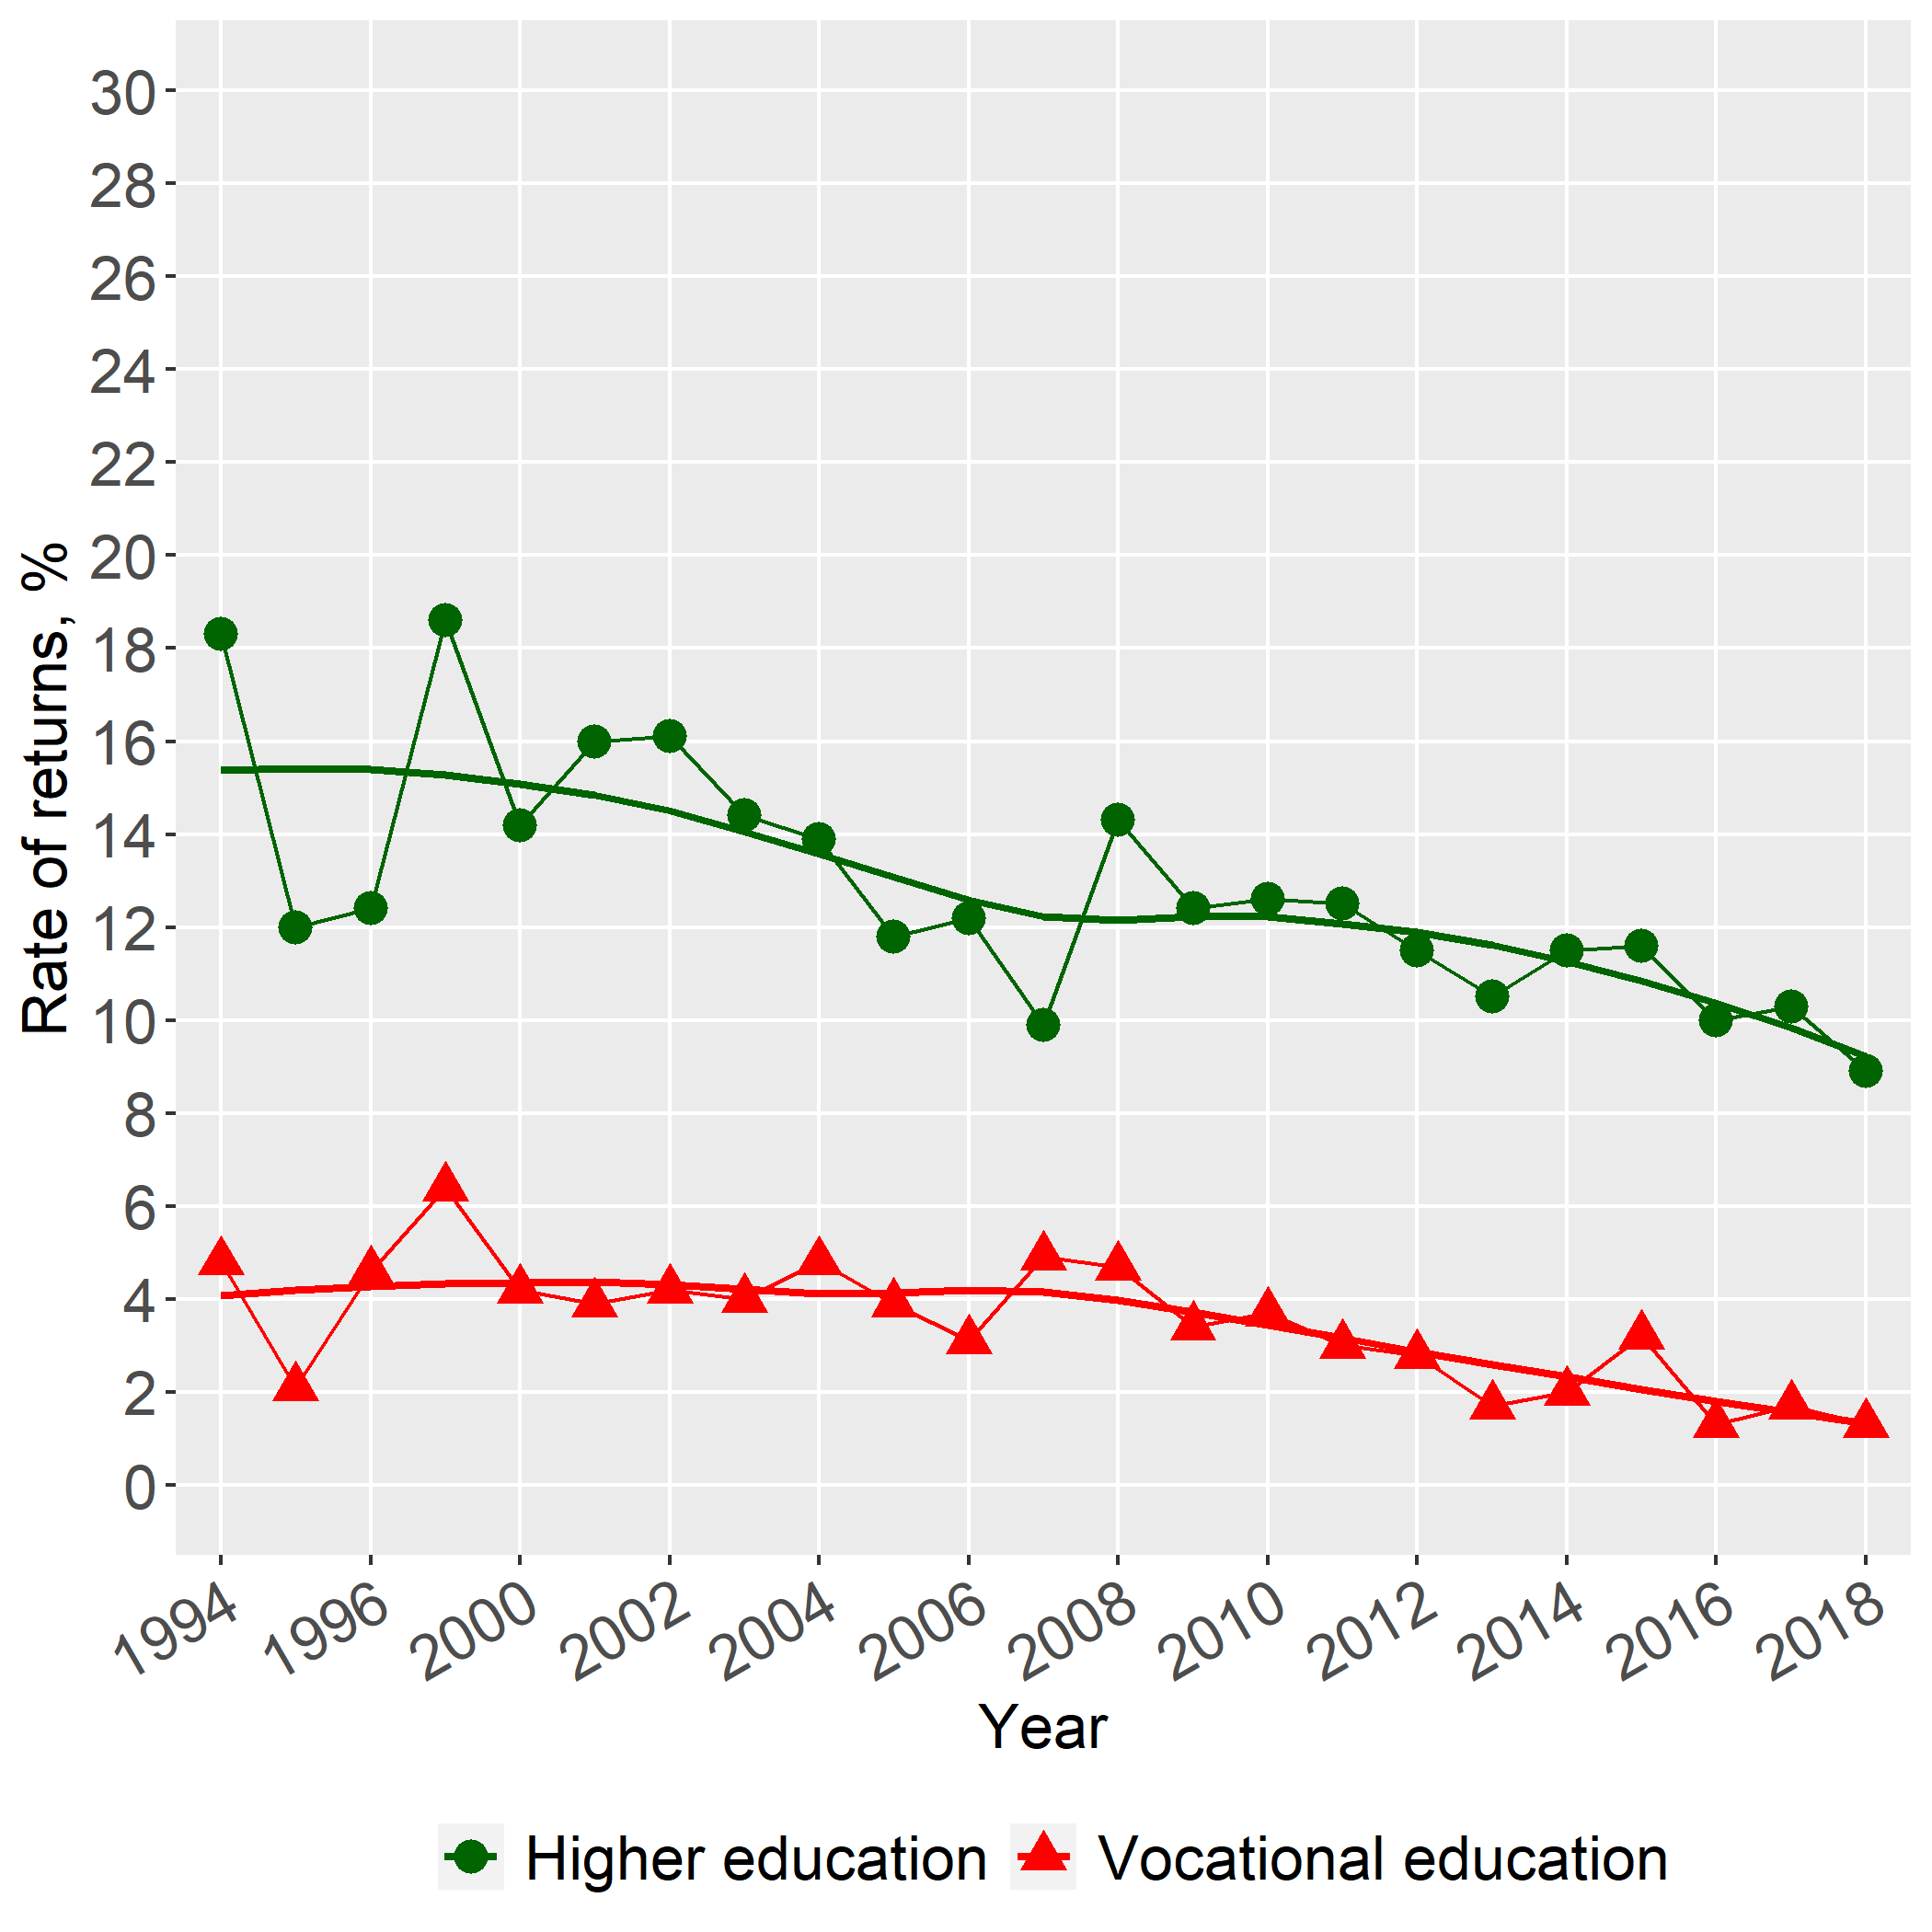
\includegraphics[width=\textwidth]{re_HE_m.png}
     % plot 2
     \subcaption{Males}\label{fig:1.4b}
  \end{minipage}
  \caption{Rates of Returns to Higher and Vocational Education in Russia, RLMS 1994-2018}\label{fig:1.4}
\end{figure}

When estimated separately by gender, we find trend variation by gender. The results from estimation of earnings functions show that annual returns to Higher education for males varied from 9\% to 15\%, whereas women's returns are described by an inversely U-shaped pattern, reaching their maximum of 28\% in 2003. Within roughly the last 5 years, wage premiums to higher education for women have stabilized at around 12\%, a couple of percentage points ahead of men.  Gender wise enrollment rates in higher education (not shown) ten years later appears to match the differences in rates of return, strengthening the hypothesis that market rates of return to education in Russia do indeed influence individual continuing school decisions. 

A similar comparative picture is observed with respect to vocational education, albeit with a different kind of variation by gender (see Figure \ref{fig:1.4}): returns for males are almost flat within the time period while returns for females shows a concave pattern. The overall outcome concerning payoffs to schooling isolated by gender has been confirmed in a similar fashion by past studies \parencite[e.g.,][]{Cheidvasser2007}.

\section{Conclusions}

This paper presents some new estimates of the returns to education in the 
Russian Federation. The estimates use a Mincerian specification common to 
one that has been carried out for over one hundred countries. The paper 
shows that Mincerian returns to higher education are three times greater 
for higher education compared to vocational education, and that the returns 
to education for females is higher than for males. 

Following expansion, the returns to schooling started to decline.

Returns for females shows an inverse U-shaped curve over the past two 
decades, but this phenomenon needs to be explored more closely
to derive policy conclusions. 


\printbibliography

\newpage

\begin{landscape}

\fontsize{9}{11}
\selectfont

\begin{table}[!htbp] \centering 
\renewcommand{\arraystretch}{1.0}
  \caption{Results of Mincer Analysis, RLMS 1994} 
  \label{} 
\begin{tabular}{@{\extracolsep{5pt}}lcccccc} 
\\[-.8ex]\hline 
\hline \\[-.8ex] 
 & Total & Males & Females & Total & Males & Females \\ 
\\[-.8ex] & (1) & (2) & (3) & (4) & (5) & (6)\\ 
\hline \\[-.8ex] 
 Constant & 10.704$^{***}$ & 10.974$^{***}$ & 10.319$^{***}$ & 11.569$^{***}$ & 11.947$^{***}$ & 11.132$^{***}$ \\ 
  & (10.435, 10.972) & (10.578, 11.369) & (9.979, 10.659) & (11.385, 11.753) & (11.673, 12.222) & (10.901, 11.362) \\ 
  & & & & & & \\ 
 Education, years & 0.084$^{***}$ & 0.094$^{***}$ & 0.082$^{***}$ &  &  &  \\ 
  & (0.069, 0.098) & (0.072, 0.115) & (0.063, 0.101) &  &  &  \\ 
  & & & & & & \\ 
 Vocational education &  &  &  & 0.114$^{***}$ & 0.135$^{**}$ & 0.156$^{***}$ \\ 
  &  &  &  & (0.029, 0.200) & (0.011, 0.260) & (0.046, 0.266) \\ 
  & & & & & & \\ 
 Higher education &  &  &  & 0.489$^{***}$ & 0.549$^{***}$ & 0.501$^{***}$ \\ 
  &  &  &  & (0.392, 0.586) & (0.407, 0.691) & (0.378, 0.625) \\ 
  & & & & & & \\ 
 Experience & 0.030$^{***}$ & 0.023$^{*}$ & 0.043$^{***}$ & 0.032$^{***}$ & 0.024$^{**}$ & 0.045$^{***}$ \\ 
  & (0.015, 0.046) & ($-$0.0002, 0.046) & (0.024, 0.062) & (0.017, 0.048) & (0.0005, 0.047) & (0.026, 0.065) \\ 
  & & & & & & \\ 
 Experience squared & $-$0.001$^{***}$ & $-$0.001$^{**}$ & $-$0.001$^{***}$ & $-$0.001$^{***}$ & $-$0.001$^{**}$ & $-$0.001$^{***}$ \\ 
  & ($-$0.001, $-$0.0003) & ($-$0.001, $-$0.0001) & ($-$0.001, $-$0.0004) & ($-$0.001, $-$0.0003) & ($-$0.001, $-$0.0001) & ($-$0.001, $-$0.0005) \\ 
  & & & & & & \\ 
\hline \\[-.8ex] 
Observations & 3,044 & 1,397 & 1,647 & 3,044 & 1,397 & 1,647 \\ 
R$^{2}$ & 0.042 & 0.055 & 0.050 & 0.041 & 0.052 & 0.049 \\ 
Adjusted R$^{2}$ & 0.041 & 0.053 & 0.048 & 0.039 & 0.049 & 0.047 \\ 
Residual Std. Error & 0.935 & 0.952 & 0.854 & 0.936 & 0.954 & 0.854 \\ 
F Statistic & 44.464$^{***}$ & 27.011$^{***}$ & 28.581$^{***}$ & 32.271$^{***}$ & 19.011$^{***}$ & 21.376$^{***}$ \\ 
\hline 
\textit{Note:}  & \multicolumn{6}{r}{$^{*}$p$<$0.1; $^{**}$p$<$0.05; $^{***}$p$<$0.01} \\ 
\end{tabular} 
\end{table} 

\end{landscape}

\newpage

\begin{landscape}

\fontsize{9}{11}
\selectfont

\begin{table}[!htbp] \centering 
\renewcommand{\arraystretch}{1.0}
  \caption{Results of Mincer Analysis, RLMS 1995} 
  \label{} 
\begin{tabular}{@{\extracolsep{5pt}}lcccccc} 
\\[-.8ex]\hline 
\hline \\[-.8ex] 
 & Total & Males & Females & Total & Males & Females \\ 
\\[-.8ex] & (1) & (2) & (3) & (4) & (5) & (6)\\ 
\hline \\[-.8ex] 
 Constant & 11.526$^{***}$ & 12.079$^{***}$ & 10.920$^{***}$ & 12.362$^{***}$ & 12.844$^{***}$ & 11.835$^{***}$ \\ 
  & (11.244, 11.808) & (11.674, 12.484) & (10.548, 11.291) & (12.172, 12.551) & (12.566, 13.121) & (11.587, 12.082) \\ 
  & & & & & & \\ 
 Education, years & 0.078$^{***}$ & 0.073$^{***}$ & 0.089$^{***}$ &  &  &  \\ 
  & (0.062, 0.094) & (0.050, 0.096) & (0.068, 0.109) &  &  &  \\ 
  & & & & & & \\ 
 Vocational education &  &  &  & 0.052 & 0.062 & 0.111$^{*}$ \\ 
  &  &  &  & ($-$0.038, 0.142) & ($-$0.067, 0.190) & ($-$0.009, 0.230) \\ 
  & & & & & & \\ 
 Higher education &  &  &  & 0.418$^{***}$ & 0.393$^{***}$ & 0.498$^{***}$ \\ 
  &  &  &  & (0.319, 0.518) & (0.251, 0.534) & (0.366, 0.631) \\ 
  & & & & & & \\ 
 Experience & 0.030$^{***}$ & 0.010 & 0.053$^{***}$ & 0.032$^{***}$ & 0.012 & 0.055$^{***}$ \\ 
  & (0.014, 0.045) & ($-$0.013, 0.033) & (0.032, 0.073) & (0.016, 0.048) & ($-$0.011, 0.035) & (0.034, 0.075) \\ 
  & & & & & & \\ 
 Experience squared & $-$0.001$^{***}$ & $-$0.0003 & $-$0.001$^{***}$ & $-$0.001$^{***}$ & $-$0.0004 & $-$0.001$^{***}$ \\ 
  & ($-$0.001, $-$0.0003) & ($-$0.001, 0.0002) & ($-$0.001, $-$0.001) & ($-$0.001, $-$0.0004) & ($-$0.001, 0.0001) & ($-$0.002, $-$0.001) \\ 
  & & & & & & \\ 
\hline \\[-.8ex] 
Observations & 2,694 & 1,238 & 1,456 & 2,694 & 1,238 & 1,456 \\ 
R$^{2}$ & 0.038 & 0.036 & 0.057 & 0.039 & 0.036 & 0.058 \\ 
Adjusted R$^{2}$ & 0.037 & 0.034 & 0.055 & 0.037 & 0.033 & 0.055 \\ 
Residual Std. Error & 0.919 & 0.920 & 0.866 & 0.919 & 0.920 & 0.866 \\ 
F Statistic & 35.479$^{***}$ & 15.338$^{***}$ & 29.289$^{***}$ & 27.160$^{***}$ & 11.401$^{***}$ & 22.178$^{***}$ \\ 
\hline 
\textit{Note:}  & \multicolumn{6}{r}{$^{*}$p$<$0.1; $^{**}$p$<$0.05; $^{***}$p$<$0.01} \\ 
\end{tabular} 
\end{table} 

\end{landscape}

\newpage

\begin{landscape}

\fontsize{9}{11}
\selectfont

\begin{table}[!htbp] \centering 
\renewcommand{\arraystretch}{1.0}
  \caption{Results of Mincer Analysis, RLMS 1996} 
  \label{} 
\begin{tabular}{@{\extracolsep{5pt}}lcccccc} 
\\[-.8ex]\hline 
\hline \\[-.8ex] 
 & Total & Males & Females & Total & Males & Females \\ 
\\[-.8ex] & (1) & (2) & (3) & (4) & (5) & (6)\\ 
\hline \\[-.8ex] 
 Constant & 12.268$^{***}$ & 12.539$^{***}$ & 11.814$^{***}$ & 12.991$^{***}$ & 13.306$^{***}$ & 12.568$^{***}$ \\ 
  & (11.947, 12.590) & (12.066, 13.013) & (11.401, 12.227) & (12.775, 13.206) & (12.987, 13.625) & (12.292, 12.843) \\ 
  & & & & & & \\ 
 Education, years & 0.071$^{***}$ & 0.076$^{***}$ & 0.074$^{***}$ &  &  &  \\ 
  & (0.052, 0.089) & (0.049, 0.103) & (0.051, 0.098) &  &  &  \\ 
  & & & & & & \\ 
 Vocational education &  &  &  & 0.104$^{*}$ & 0.130 & 0.126$^{*}$ \\ 
  &  &  &  & ($-$0.002, 0.210) & ($-$0.026, 0.286) & ($-$0.010, 0.261) \\ 
  & & & & & & \\ 
 Higher education &  &  &  & 0.380$^{***}$ & 0.403$^{***}$ & 0.412$^{***}$ \\ 
  &  &  &  & (0.265, 0.496) & (0.232, 0.574) & (0.265, 0.560) \\ 
  & & & & & & \\ 
 Experience & 0.003 & $-$0.001 & 0.018 & 0.005 & 0.001 & 0.019$^{*}$ \\ 
  & ($-$0.015, 0.020) & ($-$0.027, 0.025) & ($-$0.005, 0.040) & ($-$0.013, 0.022) & ($-$0.025, 0.027) & ($-$0.003, 0.042) \\ 
  & & & & & & \\ 
 Experience squared & $-$0.0001 & $-$0.0001 & $-$0.0004 & $-$0.0002 & $-$0.0002 & $-$0.0004$^{*}$ \\ 
  & ($-$0.001, 0.0002) & ($-$0.001, 0.0004) & ($-$0.001, 0.0001) & ($-$0.001, 0.0002) & ($-$0.001, 0.0004) & ($-$0.001, 0.0001) \\ 
  & & & & & & \\ 
\hline \\[-.8ex] 
Observations & 2,282 & 1,034 & 1,248 & 2,282 & 1,034 & 1,248 \\ 
R$^{2}$ & 0.029 & 0.037 & 0.033 & 0.026 & 0.032 & 0.031 \\ 
Adjusted R$^{2}$ & 0.027 & 0.035 & 0.031 & 0.024 & 0.028 & 0.028 \\ 
Residual Std. Error & 0.958 & 0.974 & 0.886 & 0.959 & 0.977 & 0.887 \\ 
F Statistic & 22.443$^{***}$ & 13.324$^{***}$ & 14.098$^{***}$ & 15.319$^{***}$ & 8.574$^{***}$ & 9.880$^{***}$ \\ 
\hline 
\textit{Note:}  & \multicolumn{6}{r}{$^{*}$p$<$0.1; $^{**}$p$<$0.05; $^{***}$p$<$0.01} \\ 
\end{tabular} 
\end{table} 

\end{landscape}

\newpage

\begin{landscape}

\fontsize{9}{11}
\selectfont

\begin{table}[!htbp] \centering 
\renewcommand{\arraystretch}{1.0}
  \caption{Results of Mincer Analysis, RLMS 1998} 
  \label{} 
\begin{tabular}{@{\extracolsep{5pt}}lcccccc} 
\\[-.8ex]\hline 
\hline \\[-.8ex] 
 & Total & Males & Females & Total & Males & Females \\ 
\\[-.8ex] & (1) & (2) & (3) & (4) & (5) & (6)\\ 
\hline \\[-.8ex] 
 Constant & 5.118$^{***}$ & 5.425$^{***}$ & 4.564$^{***}$ & 5.963$^{***}$ & 6.338$^{***}$ & 5.502$^{***}$ \\ 
  & (4.885, 5.350) & (5.090, 5.760) & (4.267, 4.861) & (5.805, 6.120) & (6.106, 6.571) & (5.303, 5.700) \\ 
  & & & & & & \\ 
 Education, years & 0.088$^{***}$ & 0.095$^{***}$ & 0.099$^{***}$ &  &  &  \\ 
  & (0.075, 0.101) & (0.076, 0.114) & (0.083, 0.116) &  &  &  \\ 
  & & & & & & \\ 
 Vocational education &  &  &  & 0.177$^{***}$ & 0.175$^{***}$ & 0.257$^{***}$ \\ 
  &  &  &  & (0.102, 0.252) & (0.070, 0.280) & (0.158, 0.355) \\ 
  & & & & & & \\ 
 Higher education &  &  &  & 0.528$^{***}$ & 0.556$^{***}$ & 0.615$^{***}$ \\ 
  &  &  &  & (0.444, 0.613) & (0.435, 0.677) & (0.506, 0.725) \\ 
  & & & & & & \\ 
 Experience & 0.024$^{***}$ & 0.013 & 0.041$^{***}$ & 0.028$^{***}$ & 0.018$^{*}$ & 0.043$^{***}$ \\ 
  & (0.012, 0.037) & ($-$0.005, 0.032) & (0.025, 0.057) & (0.015, 0.040) & ($-$0.001, 0.037) & (0.027, 0.059) \\ 
  & & & & & & \\ 
 Experience squared & $-$0.001$^{***}$ & $-$0.0004$^{*}$ & $-$0.001$^{***}$ & $-$0.001$^{***}$ & $-$0.0005$^{**}$ & $-$0.001$^{***}$ \\ 
  & ($-$0.001, $-$0.0003) & ($-$0.001, 0.00003) & ($-$0.001, $-$0.001) & ($-$0.001, $-$0.0003) & ($-$0.001, $-$0.0001) & ($-$0.001, $-$0.001) \\ 
  & & & & & & \\ 
\hline \\[-.8ex] 
Observations & 3,102 & 1,434 & 1,668 & 3,102 & 1,434 & 1,668 \\ 
R$^{2}$ & 0.057 & 0.069 & 0.085 & 0.058 & 0.067 & 0.085 \\ 
Adjusted R$^{2}$ & 0.056 & 0.067 & 0.083 & 0.057 & 0.064 & 0.083 \\ 
Residual Std. Error & 0.800 & 0.803 & 0.730 & 0.800 & 0.804 & 0.730 \\ 
F Statistic & 62.558$^{***}$ & 35.348$^{***}$ & 51.380$^{***}$ & 47.536$^{***}$ & 25.536$^{***}$ & 38.668$^{***}$ \\ 
\hline 
\textit{Note:}  & \multicolumn{6}{r}{$^{*}$p$<$0.1; $^{**}$p$<$0.05; $^{***}$p$<$0.01} \\ 
\end{tabular} 
\end{table} 

\end{landscape}

\newpage

\begin{landscape}
	
	\fontsize{9}{11}
	\selectfont
	
	\begin{table}[!htbp] \centering 
\renewcommand{\arraystretch}{1.0}
		\caption{Results of Mincer Analysis, RLMS 2000} 
		\label{} 
		\begin{tabular}{@{\extracolsep{5pt}}lcccccc} 
			\\[-.8ex]\hline 
			\hline \\[-.8ex] 
			& Total & Males & Females & Total & Males & Females \\ 
			\\[-.8ex] & (1) & (2) & (3) & (4) & (5) & (6)\\ 
			\hline \\[-.8ex] 
			Constant & 5.834$^{***}$ & 6.311$^{***}$ & 5.023$^{***}$ & 6.700$^{***}$ & 7.183$^{***}$ & 6.072$^{***}$ \\ 
			& (5.591, 6.077) & (5.966, 6.655) & (4.710, 5.336) & (6.543, 6.857) & (6.961, 7.405) & (5.869, 6.276) \\ 
			& & & & & & \\ 
			Education, years & 0.087$^{***}$ & 0.086$^{***}$ & 0.110$^{***}$ &  &  &  \\ 
			& (0.072, 0.101) & (0.065, 0.106) & (0.092, 0.128) &  &  &  \\ 
			& & & & & & \\ 
			Vocational education &  &  &  & 0.153$^{***}$ & 0.118$^{**}$ & 0.283$^{***}$ \\ 
			&  &  &  & (0.073, 0.233) & (0.008, 0.228) & (0.178, 0.388) \\ 
			& & & & & & \\ 
			Higher education &  &  &  & 0.488$^{***}$ & 0.450$^{***}$ & 0.668$^{***}$ \\ 
			&  &  &  & (0.398, 0.577) & (0.323, 0.578) & (0.553, 0.784) \\ 
			& & & & & & \\ 
			Experience & 0.019$^{***}$ & 0.006 & 0.041$^{***}$ & 0.021$^{***}$ & 0.009 & 0.042$^{***}$ \\ 
			& (0.006, 0.032) & ($-$0.012, 0.025) & (0.024, 0.057) & (0.008, 0.034) & ($-$0.009, 0.028) & (0.025, 0.058) \\ 
			& & & & & & \\ 
			Experience squared & $-$0.0004$^{***}$ & $-$0.0002 & $-$0.001$^{***}$ & $-$0.0005$^{***}$ & $-$0.0003$^{*}$ & $-$0.001$^{***}$ \\ 
			& ($-$0.001, $-$0.0001) & ($-$0.001, 0.0001) & ($-$0.001, $-$0.0004) & ($-$0.001, $-$0.0002) & ($-$0.001, 0.0001) & ($-$0.001, $-$0.0005) \\ 
			& & & & & & \\ 
			\hline \\[-.8ex] 
			Observations & 3,215 & 1,477 & 1,738 & 3,215 & 1,477 & 1,738 \\ 
			R$^{2}$ & 0.047 & 0.053 & 0.084 & 0.044 & 0.047 & 0.082 \\ 
			Adjusted R$^{2}$ & 0.046 & 0.051 & 0.082 & 0.043 & 0.044 & 0.080 \\ 
			Residual Std. Error & 0.867 & 0.856 & 0.796 & 0.869 & 0.859 & 0.797 \\ 
			F Statistic & 52.584$^{***}$ & 27.384$^{***}$ & 53.004$^{***}$ & 36.873$^{***}$ & 17.961$^{***}$ & 38.813$^{***}$ \\ 
			\hline 

			\textit{Note:}  & \multicolumn{6}{r}{$^{*}$p$<$0.1; $^{**}$p$<$0.05; $^{***}$p$<$0.01} \\ 
		\end{tabular} 
	\end{table} 
	
\end{landscape}

\newpage

\begin{landscape}
	
	\fontsize{9}{11}
	\selectfont
	
	\begin{table}[!htbp] \centering 
\renewcommand{\arraystretch}{1.0}
		\caption{Results of Mincer Analysis, RLMS 2001} 
		\label{} 
		\begin{tabular}{@{\extracolsep{5pt}}lcccccc} 
			\\[-.8ex]\hline 
			\hline \\[-.8ex] 
			& Total & Males & Females & Total & Males & Females \\ 
			\\[-.8ex] & (1) & (2) & (3) & (4) & (5) & (6)\\ 
			\hline \\[-.8ex] 
			Constant & 6.343$^{***}$ & 6.648$^{***}$ & 5.647$^{***}$ & 7.287$^{***}$ & 7.592$^{***}$ & 6.758$^{***}$ \\ 
			& (6.120, 6.566) & (6.329, 6.968) & (5.355, 5.939) & (7.143, 7.430) & (7.389, 7.795) & (6.569, 6.947) \\ 
			& & & & & & \\ 
			Education, years & 0.093$^{***}$ & 0.092$^{***}$ & 0.116$^{***}$ &  &  &  \\ 
			& (0.080, 0.106) & (0.073, 0.111) & (0.099, 0.132) &  &  &  \\ 
			& & & & & & \\ 
			Vocational education &  &  &  & 0.144$^{***}$ & 0.111$^{**}$ & 0.293$^{***}$ \\ 
			&  &  &  & (0.070, 0.218) & (0.008, 0.213) & (0.193, 0.393) \\ 
			& & & & & & \\ 
			Higher education &  &  &  & 0.519$^{***}$ & 0.496$^{***}$ & 0.711$^{***}$ \\ 
			&  &  &  & (0.438, 0.600) & (0.380, 0.612) & (0.603, 0.819) \\ 
			& & & & & & \\ 
			Experience & 0.001 & 0.001 & 0.013 & 0.003 & 0.004 & 0.013 \\ 
			& ($-$0.011, 0.013) & ($-$0.016, 0.018) & ($-$0.003, 0.029) & ($-$0.009, 0.015) & ($-$0.014, 0.021) & ($-$0.003, 0.029) \\ 
			& & & & & & \\ 
			Experience squared & $-$0.0001 & $-$0.0001 & $-$0.0002 & $-$0.0001 & $-$0.0002 & $-$0.0002 \\ 
			& ($-$0.0003, 0.0002) & ($-$0.0005, 0.0002) & ($-$0.001, 0.0001) & ($-$0.0004, 0.0001) & ($-$0.001, 0.0002) & ($-$0.001, 0.0001) \\ 
			& & & & & & \\ 
			\hline \\[-.8ex] 
			Observations & 3,605 & 1,673 & 1,932 & 3,605 & 1,673 & 1,932 \\ 
			R$^{2}$ & 0.057 & 0.060 & 0.090 & 0.056 & 0.057 & 0.092 \\ 
			Adjusted R$^{2}$ & 0.056 & 0.058 & 0.088 & 0.054 & 0.055 & 0.090 \\ 
			Residual Std. Error & 0.844 & 0.851 & 0.774 & 0.844 & 0.852 & 0.773 \\ 
			F Statistic & 72.009$^{***}$ & 35.323$^{***}$ & 63.474$^{***}$ & 52.935$^{***}$ & 25.340$^{***}$ & 48.998$^{***}$ \\ 
			\hline 
			\textit{Note:}  & \multicolumn{6}{r}{$^{*}$p$<$0.1; $^{**}$p$<$0.05; $^{***}$p$<$0.01} \\ 
		\end{tabular} 
	\end{table} 
	
\end{landscape}

\newpage

\begin{landscape}
	
	\fontsize{9}{11}
	\selectfont
	
	\begin{table}[!htbp] \centering 
\renewcommand{\arraystretch}{1.0}
		\caption{Results of Mincer Analysis, RLMS 2002} 
		\label{} 
		\begin{tabular}{@{\extracolsep{5pt}}lcccccc} 
			\\[-.8ex]\hline 
			\hline \\[-.8ex] 
			& Total & Males & Females & Total & Males & Females \\ 
			\\[-.8ex] & (1) & (2) & (3) & (4) & (5) & (6)\\ 
			\hline \\[-.8ex] 
			Constant & 6.547$^{***}$ & 6.852$^{***}$ & 5.884$^{***}$ & 7.469$^{***}$ & 7.795$^{***}$ & 6.957$^{***}$ \\ 
			& (6.346, 6.748) & (6.567, 7.137) & (5.620, 6.147) & (7.340, 7.598) & (7.614, 7.976) & (6.785, 7.129) \\ 
			& & & & & & \\ 
			Education, years & 0.092$^{***}$ & 0.093$^{***}$ & 0.113$^{***}$ &  &  &  \\ 
			& (0.080, 0.104) & (0.076, 0.111) & (0.098, 0.128) &  &  &  \\ 
			& & & & & & \\ 
			Vocational education &  &  &  & 0.147$^{***}$ & 0.120$^{**}$ & 0.283$^{***}$ \\ 
			&  &  &  & (0.080, 0.214) & (0.028, 0.211) & (0.192, 0.374) \\ 
			& & & & & & \\ 
			Higher education &  &  &  & 0.511$^{***}$ & 0.498$^{***}$ & 0.686$^{***}$ \\ 
			&  &  &  & (0.437, 0.584) & (0.394, 0.602) & (0.588, 0.784) \\ 
			& & & & & & \\ 
			Experience & 0.015$^{***}$ & 0.012 & 0.028$^{***}$ & 0.018$^{***}$ & 0.016$^{**}$ & 0.029$^{***}$ \\ 
			& (0.005, 0.026) & ($-$0.003, 0.028) & (0.014, 0.042) & (0.007, 0.029) & (0.001, 0.032) & (0.014, 0.043) \\ 
			& & & & & & \\ 
			Experience squared & $-$0.0003$^{***}$ & $-$0.0004$^{**}$ & $-$0.0005$^{***}$ & $-$0.0004$^{***}$ & $-$0.0005$^{***}$ & $-$0.0005$^{***}$ \\ 
			& ($-$0.001, $-$0.0001) & ($-$0.001, $-$0.0001) & ($-$0.001, $-$0.0002) & ($-$0.001, $-$0.0002) & ($-$0.001, $-$0.0001) & ($-$0.001, $-$0.0002) \\ 
			& & & & & & \\ 
			\hline \\[-.8ex] 
			Observations & 3,803 & 1,748 & 2,055 & 3,803 & 1,748 & 2,055 \\ 
			R$^{2}$ & 0.062 & 0.072 & 0.098 & 0.060 & 0.068 & 0.099 \\ 
			Adjusted R$^{2}$ & 0.061 & 0.071 & 0.097 & 0.059 & 0.066 & 0.097 \\ 
			Residual Std. Error & 0.777 & 0.770 & 0.722 & 0.778 & 0.771 & 0.722 \\ 
			F Statistic & 84.039$^{***}$ & 45.377$^{***}$ & 74.224$^{***}$ & 60.863$^{***}$ & 31.968$^{***}$ & 56.066$^{***}$ \\ 
			\hline 
			\textit{Note:}  & \multicolumn{6}{r}{$^{*}$p$<$0.1; $^{**}$p$<$0.05; $^{***}$p$<$0.01} \\ 
		\end{tabular} 
	\end{table} 
	
\end{landscape}

\newpage

\begin{landscape}
	
	\fontsize{9}{11}
	\selectfont
	
	\begin{table}[!htbp] \centering 
\renewcommand{\arraystretch}{1.0}
		\caption{Results of Mincer Analysis, RLMS 2003} 
		\label{} 
		\begin{tabular}{@{\extracolsep{5pt}}lcccccc} 
			\\[-.8ex]\hline 
			\hline \\[-.8ex] 
			& Total & Males & Females & Total & Males & Females \\ 
			\\[-.8ex] & (1) & (2) & (3) & (4) & (5) & (6)\\ 
			\hline \\[-.8ex] 
			Constant & 6.779$^{***}$ & 7.204$^{***}$ & 6.054$^{***}$ & 7.695$^{***}$ & 8.127$^{***}$ & 7.167$^{***}$ \\ 
			& (6.578, 6.979) & (6.922, 7.486) & (5.793, 6.315) & (7.567, 7.824) & (7.945, 8.308) & (7.001, 7.333) \\ 
			& & & & & & \\ 
			Education, years & 0.093$^{***}$ & 0.089$^{***}$ & 0.119$^{***}$ &  &  &  \\ 
			& (0.081, 0.104) & (0.073, 0.106) & (0.104, 0.134) &  &  &  \\ 
			& & & & & & \\ 
			Vocational education &  &  &  & 0.169$^{***}$ & 0.114$^{**}$ & 0.323$^{***}$ \\ 
			&  &  &  & (0.102, 0.237) & (0.023, 0.204) & (0.232, 0.414) \\ 
			& & & & & & \\ 
			Higher education &  &  &  & 0.520$^{***}$ & 0.456$^{***}$ & 0.740$^{***}$ \\ 
			&  &  &  & (0.447, 0.594) & (0.353, 0.558) & (0.642, 0.838) \\ 
			& & & & & & \\ 
			Experience & 0.016$^{***}$ & 0.009 & 0.025$^{***}$ & 0.018$^{***}$ & 0.011 & 0.025$^{***}$ \\ 
			& (0.005, 0.026) & ($-$0.007, 0.024) & (0.011, 0.038) & (0.007, 0.029) & ($-$0.005, 0.027) & (0.011, 0.039) \\ 
			& & & & & & \\ 
			Experience squared & $-$0.0004$^{***}$ & $-$0.0004$^{**}$ & $-$0.0005$^{***}$ & $-$0.0004$^{***}$ & $-$0.0004$^{**}$ & $-$0.0005$^{***}$ \\ 
			& ($-$0.001, $-$0.0002) & ($-$0.001, $-$0.00002) & ($-$0.001, $-$0.0002) & ($-$0.001, $-$0.0002) & ($-$0.001, $-$0.0001) & ($-$0.001, $-$0.0002) \\ 
			& & & & & & \\ 
			\hline \\[-.8ex] 
			Observations & 3,858 & 1,765 & 2,093 & 3,858 & 1,765 & 2,093 \\ 
			R$^{2}$ & 0.068 & 0.078 & 0.107 & 0.065 & 0.069 & 0.110 \\ 
			Adjusted R$^{2}$ & 0.067 & 0.077 & 0.106 & 0.064 & 0.067 & 0.108 \\ 
			Residual Std. Error & 0.782 & 0.753 & 0.732 & 0.783 & 0.757 & 0.731 \\ 
			F Statistic & 93.289$^{***}$ & 49.918$^{***}$ & 83.800$^{***}$ & 66.602$^{***}$ & 32.690$^{***}$ & 64.384$^{***}$ \\ 
			\hline 
			\textit{Note:}  & \multicolumn{6}{r}{$^{*}$p$<$0.1; $^{**}$p$<$0.05; $^{***}$p$<$0.01} \\ 
		\end{tabular} 
	\end{table} 
	
\end{landscape}

\newpage

\begin{landscape}
	
	\fontsize{9}{11}
	\selectfont
	
	\begin{table}[!htbp] \centering 
\renewcommand{\arraystretch}{1.0}
		\caption{Results of Mincer Analysis, RLMS 2004} 
		\label{} 
		\begin{tabular}{@{\extracolsep{5pt}}lcccccc} 
			\\[-.8ex]\hline 
			\hline \\[-.8ex] 
			& Total & Males & Females & Total & Males & Females \\ 
			\\[-.8ex] & (1) & (2) & (3) & (4) & (5) & (6)\\ 
			\hline \\[-.8ex] 
			Constant & 7.181$^{***}$ & 7.559$^{***}$ & 6.437$^{***}$ & 8.053$^{***}$ & 8.404$^{***}$ & 7.553$^{***}$ \\ 
			& (6.990, 7.371) & (7.293, 7.825) & (6.191, 6.683) & (7.931, 8.174) & (8.233, 8.574) & (7.397, 7.710) \\ 
			& & & & & & \\ 
			Education, years & 0.085$^{***}$ & 0.084$^{***}$ & 0.111$^{***}$ &  &  &  \\ 
			& (0.074, 0.096) & (0.068, 0.099) & (0.097, 0.125) &  &  &  \\ 
			& & & & & & \\ 
			Vocational education &  &  &  & 0.105$^{***}$ & 0.135$^{***}$ & 0.180$^{***}$ \\ 
			&  &  &  & (0.041, 0.170) & (0.050, 0.221) & (0.093, 0.267) \\ 
			& & & & & & \\ 
			Higher education &  &  &  & 0.445$^{***}$ & 0.443$^{***}$ & 0.610$^{***}$ \\ 
			&  &  &  & (0.374, 0.516) & (0.345, 0.540) & (0.516, 0.704) \\ 
			& & & & & & \\ 
			Experience & 0.011$^{**}$ & 0.005 & 0.022$^{***}$ & 0.013$^{**}$ & 0.007 & 0.024$^{***}$ \\ 
			& (0.0003, 0.021) & ($-$0.009, 0.020) & (0.009, 0.035) & (0.003, 0.023) & ($-$0.007, 0.022) & (0.011, 0.038) \\ 
			& & & & & & \\ 
			Experience squared & $-$0.0003$^{***}$ & $-$0.0003$^{*}$ & $-$0.0005$^{***}$ & $-$0.0004$^{***}$ & $-$0.0004$^{**}$ & $-$0.001$^{***}$ \\ 
			& ($-$0.001, $-$0.0001) & ($-$0.001, 0.00000) & ($-$0.001, $-$0.0002) & ($-$0.001, $-$0.0002) & ($-$0.001, $-$0.00005) & ($-$0.001, $-$0.0002) \\ 
			& & & & & & \\ 
			\hline \\[-.8ex] 
			Observations & 3,968 & 1,824 & 2,144 & 3,968 & 1,824 & 2,144 \\ 
			R$^{2}$ & 0.068 & 0.084 & 0.106 & 0.063 & 0.075 & 0.101 \\ 
			Adjusted R$^{2}$ & 0.067 & 0.083 & 0.105 & 0.062 & 0.073 & 0.099 \\ 
			Residual Std. Error & 0.748 & 0.720 & 0.690 & 0.750 & 0.724 & 0.693 \\ 
			F Statistic & 96.254$^{***}$ & 55.701$^{***}$ & 84.918$^{***}$ & 66.116$^{***}$ & 36.626$^{***}$ & 59.781$^{***}$ \\ 
			\hline 
			\textit{Note:}  & \multicolumn{6}{r}{$^{*}$p$<$0.1; $^{**}$p$<$0.05; $^{***}$p$<$0.01} \\ 
		\end{tabular} 
	\end{table} 
	
\end{landscape}

\newpage

\begin{landscape}
	
	\fontsize{9}{11}
	\selectfont
	
	\begin{table}[!htbp] \centering 
\renewcommand{\arraystretch}{1.0}
		\caption{Results of Mincer Analysis, RLMS 2005} 
		\label{} 
		\begin{tabular}{@{\extracolsep{5pt}}lcccccc} 
			\\[-.8ex]\hline 
			\hline \\[-.8ex] 
			& Total & Males & Females & Total & Males & Females \\ 
			\\[-.8ex] & (1) & (2) & (3) & (4) & (5) & (6)\\ 
			\hline \\[-.8ex] 
			Constant & 7.541$^{***}$ & 7.969$^{***}$ & 6.729$^{***}$ & 8.374$^{***}$ & 8.722$^{***}$ & 7.868$^{***}$ \\ 
			& (7.352, 7.731) & (7.703, 8.235) & (6.485, 6.972) & (8.255, 8.494) & (8.555, 8.890) & (7.715, 8.021) \\ 
			& & & & & & \\ 
			Education, years & 0.081$^{***}$ & 0.074$^{***}$ & 0.113$^{***}$ &  &  &  \\ 
			& (0.069, 0.092) & (0.059, 0.090) & (0.099, 0.127) &  &  &  \\ 
			& & & & & & \\ 
			Vocational education &  &  &  & 0.083$^{**}$ & 0.110$^{**}$ & 0.189$^{***}$ \\ 
			&  &  &  & (0.019, 0.147) & (0.026, 0.195) & (0.101, 0.277) \\ 
			& & & & & & \\ 
			Higher education &  &  &  & 0.421$^{***}$ & 0.388$^{***}$ & 0.640$^{***}$ \\ 
			&  &  &  & (0.351, 0.492) & (0.291, 0.484) & (0.546, 0.734) \\ 
			& & & & & & \\ 
			Experience & 0.001 & $-$0.004 & 0.011$^{*}$ & 0.004 & $-$0.002 & 0.013$^{**}$ \\ 
			& ($-$0.008, 0.011) & ($-$0.018, 0.010) & ($-$0.001, 0.024) & ($-$0.006, 0.014) & ($-$0.016, 0.013) & (0.0004, 0.025) \\ 
			& & & & & & \\ 
			Experience squared & $-$0.0001 & $-$0.0001 & $-$0.0003$^{*}$ & $-$0.0002$^{*}$ & $-$0.0001 & $-$0.0003$^{**}$ \\ 
			& ($-$0.0004, 0.0001) & ($-$0.0004, 0.0002) & ($-$0.001, 0.00001) & ($-$0.0004, 0.00001) & ($-$0.0004, 0.0002) & ($-$0.001, $-$0.00001) \\ 
			& & & & & & \\ 
			\hline \\[-.8ex] 
			Observations & 3,913 & 1,801 & 2,112 & 3,913 & 1,801 & 2,112 \\ 
			R$^{2}$ & 0.065 & 0.069 & 0.116 & 0.062 & 0.061 & 0.113 \\ 
			Adjusted R$^{2}$ & 0.064 & 0.067 & 0.114 & 0.061 & 0.059 & 0.111 \\ 
			Residual Std. Error & 0.744 & 0.716 & 0.685 & 0.745 & 0.719 & 0.686 \\ 
			F Statistic & 89.991$^{***}$ & 44.143$^{***}$ & 91.939$^{***}$ & 64.154$^{***}$ & 29.157$^{***}$ & 67.046$^{***}$ \\ 
			\hline 
			\textit{Note:}  & \multicolumn{6}{r}{$^{*}$p$<$0.1; $^{**}$p$<$0.05; $^{***}$p$<$0.01} \\ 
		\end{tabular} 
	\end{table} 
	
\end{landscape}

\newpage

\begin{landscape}
	
	\fontsize{9}{11}
	\selectfont
	
	\begin{table}[!htbp] \centering 
\renewcommand{\arraystretch}{1.0}
		\caption{Results of Mincer Analysis, RLMS 2006} 
		\label{} 
		\begin{tabular}{@{\extracolsep{5pt}}lcccccc} 
			\\[-.8ex]\hline 
			\hline \\[-.8ex] 
			& Total & Males & Females & Total & Males & Females \\ 
			\\[-.8ex] & (1) & (2) & (3) & (4) & (5) & (6)\\ 
			\hline \\[-.8ex] 
			Constant & 7.764$^{***}$ & 8.149$^{***}$ & 7.011$^{***}$ & 8.596$^{***}$ & 8.878$^{***}$ & 8.173$^{***}$ \\ 
			& (7.601, 7.926) & (7.917, 8.381) & (6.804, 7.218) & (8.492, 8.700) & (8.729, 9.026) & (8.039, 8.306) \\ 
			& & & & & & \\ 
			Education, years & 0.080$^{***}$ & 0.072$^{***}$ & 0.114$^{***}$ &  &  &  \\ 
			& (0.071, 0.090) & (0.058, 0.085) & (0.102, 0.126) &  &  &  \\ 
			& & & & & & \\ 
			Vocational education &  &  &  & 0.081$^{***}$ & 0.090$^{**}$ & 0.196$^{***}$ \\ 
			&  &  &  & (0.026, 0.137) & (0.016, 0.164) & (0.119, 0.274) \\ 
			& & & & & & \\ 
			Higher education &  &  &  & 0.443$^{***}$ & 0.397$^{***}$ & 0.658$^{***}$ \\ 
			&  &  &  & (0.381, 0.504) & (0.312, 0.482) & (0.575, 0.741) \\ 
			& & & & & & \\ 
			Experience & 0.003 & 0.003 & 0.010$^{*}$ & 0.005 & 0.005 & 0.010$^{*}$ \\ 
			& ($-$0.005, 0.012) & ($-$0.010, 0.016) & ($-$0.001, 0.021) & ($-$0.003, 0.014) & ($-$0.008, 0.017) & ($-$0.001, 0.021) \\ 
			& & & & & & \\ 
			Experience squared & $-$0.0002$^{**}$ & $-$0.0002$^{*}$ & $-$0.0003$^{**}$ & $-$0.0003$^{***}$ & $-$0.0003$^{**}$ & $-$0.0003$^{**}$ \\ 
			& ($-$0.0004, $-$0.00004) & ($-$0.001, 0.00002) & ($-$0.001, $-$0.0001) & ($-$0.0005, $-$0.0001) & ($-$0.001, $-$0.00002) & ($-$0.001, $-$0.0001) \\ 
			& & & & & & \\ 
			\hline \\[-.8ex] 
			Observations & 4,804 & 2,172 & 2,632 & 4,804 & 2,172 & 2,632 \\ 
			R$^{2}$ & 0.078 & 0.074 & 0.140 & 0.078 & 0.072 & 0.134 \\ 
			Adjusted R$^{2}$ & 0.077 & 0.073 & 0.139 & 0.077 & 0.070 & 0.132 \\ 
			Residual Std. Error & 0.715 & 0.688 & 0.664 & 0.715 & 0.689 & 0.666 \\ 
			F Statistic & 135.305$^{***}$ & 58.011$^{***}$ & 142.254$^{***}$ & 101.846$^{***}$ & 41.810$^{***}$ & 101.410$^{***}$ \\ 
			\hline 
			\textit{Note:}  & \multicolumn{6}{r}{$^{*}$p$<$0.1; $^{**}$p$<$0.05; $^{***}$p$<$0.01} \\ 
		\end{tabular} 
	\end{table} 
	
\end{landscape}

\newpage

\begin{landscape}
	
	\fontsize{9}{11}
	\selectfont
	
	\begin{table}[!htbp] \centering 
\renewcommand{\arraystretch}{1.0}
		\caption{Results of Mincer Analysis, RLMS 2007} 
		\label{} 
		\begin{tabular}{@{\extracolsep{5pt}}lcccccc} 
			\\[-.8ex]\hline 
			\hline \\[-.8ex] 
			& Total & Males & Females & Total & Males & Females \\ 
			\\[-.8ex] & (1) & (2) & (3) & (4) & (5) & (6)\\ 
			\hline \\[-.8ex] 
			Constant & 8.165$^{***}$ & 8.530$^{***}$ & 7.461$^{***}$ & 8.840$^{***}$ & 9.099$^{***}$ & 8.461$^{***}$ \\ 
			& (8.009, 8.320) & (8.312, 8.747) & (7.258, 7.663) & (8.742, 8.939) & (8.961, 9.237) & (8.333, 8.588) \\ 
			& & & & & & \\ 
			Education, years & 0.066$^{***}$ & 0.058$^{***}$ & 0.097$^{***}$ &  &  &  \\ 
			& (0.057, 0.075) & (0.045, 0.070) & (0.085, 0.108) &  &  &  \\ 
			& & & & & & \\ 
			Vocational education &  &  &  & 0.083$^{***}$ & 0.136$^{***}$ & 0.138$^{***}$ \\ 
			&  &  &  & (0.030, 0.135) & (0.068, 0.204) & (0.064, 0.211) \\ 
			& & & & & & \\ 
			Higher education &  &  &  & 0.370$^{***}$ & 0.334$^{***}$ & 0.543$^{***}$ \\ 
			&  &  &  & (0.312, 0.427) & (0.256, 0.413) & (0.465, 0.622) \\ 
			& & & & & & \\ 
			Experience & 0.004 & 0.003 & 0.011$^{**}$ & 0.005 & 0.002 & 0.012$^{**}$ \\ 
			& ($-$0.004, 0.013) & ($-$0.009, 0.014) & (0.001, 0.022) & ($-$0.003, 0.014) & ($-$0.010, 0.014) & (0.002, 0.023) \\ 
			& & & & & & \\ 
			Experience squared & $-$0.0003$^{***}$ & $-$0.0003$^{**}$ & $-$0.0003$^{***}$ & $-$0.0003$^{***}$ & $-$0.0002$^{*}$ & $-$0.0004$^{***}$ \\ 
			& ($-$0.0004, $-$0.0001) & ($-$0.0005, $-$0.00001) & ($-$0.001, $-$0.0001) & ($-$0.0005, $-$0.0001) & ($-$0.0005, 0.00001) & ($-$0.001, $-$0.0001) \\ 
			& & & & & & \\ 
			\hline \\[-.8ex] 
			Observations & 4,726 & 2,153 & 2,573 & 4,726 & 2,153 & 2,573 \\ 
			R$^{2}$ & 0.070 & 0.070 & 0.121 & 0.070 & 0.066 & 0.119 \\ 
			Adjusted R$^{2}$ & 0.069 & 0.069 & 0.120 & 0.069 & 0.064 & 0.118 \\ 
			Residual Std. Error & 0.670 & 0.634 & 0.633 & 0.670 & 0.635 & 0.634 \\ 
			F Statistic & 118.364$^{***}$ & 54.316$^{***}$ & 117.362$^{***}$ & 88.551$^{***}$ & 38.060$^{***}$ & 86.643$^{***}$ \\ 
			\hline 
			\textit{Note:}  & \multicolumn{6}{r}{$^{*}$p$<$0.1; $^{**}$p$<$0.05; $^{***}$p$<$0.01} \\ 
		\end{tabular} 
	\end{table} 
	
\end{landscape}

\newpage

\begin{landscape}
	
	\fontsize{9}{11}
	\selectfont
	
	\begin{table}[!htbp] \centering 
\renewcommand{\arraystretch}{1.0}
		\caption{Results of Mincer Analysis, RLMS 2008} 
		\label{} 
		\begin{tabular}{@{\extracolsep{5pt}}lcccccc} 
			\\[-.8ex]\hline 
			\hline \\[-.8ex] 
			& Total & Males & Females & Total & Males & Females \\ 
			\\[-.8ex] & (1) & (2) & (3) & (4) & (5) & (6)\\ 
			\hline \\[-.8ex] 
			Constant & 8.134$^{***}$ & 8.412$^{***}$ & 7.473$^{***}$ & 8.918$^{***}$ & 9.146$^{***}$ & 8.549$^{***}$ \\ 
			& (7.969, 8.299) & (8.178, 8.646) & (7.260, 7.686) & (8.814, 9.022) & (9.000, 9.292) & (8.414, 8.684) \\ 
			& & & & & & \\ 
			Education, years & 0.079$^{***}$ & 0.077$^{***}$ & 0.108$^{***}$ &  &  &  \\ 
			& (0.069, 0.088) & (0.063, 0.090) & (0.096, 0.120) &  &  &  \\ 
			& & & & & & \\ 
			Vocational education &  &  &  & 0.097$^{***}$ & 0.133$^{***}$ & 0.178$^{***}$ \\ 
			&  &  &  & (0.041, 0.153) & (0.060, 0.206) & (0.099, 0.257) \\ 
			& & & & & & \\ 
			Higher education &  &  &  & 0.443$^{***}$ & 0.453$^{***}$ & 0.608$^{***}$ \\ 
			&  &  &  & (0.382, 0.504) & (0.370, 0.537) & (0.524, 0.692) \\ 
			& & & & & & \\ 
			Experience & 0.016$^{***}$ & 0.018$^{***}$ & 0.018$^{***}$ & 0.018$^{***}$ & 0.021$^{***}$ & 0.020$^{***}$ \\ 
			& (0.007, 0.024) & (0.006, 0.031) & (0.008, 0.029) & (0.010, 0.027) & (0.008, 0.033) & (0.009, 0.031) \\ 
			& & & & & & \\ 
			Experience squared & $-$0.0005$^{***}$ & $-$0.001$^{***}$ & $-$0.0005$^{***}$ & $-$0.001$^{***}$ & $-$0.001$^{***}$ & $-$0.001$^{***}$ \\ 
			& ($-$0.001, $-$0.0003) & ($-$0.001, $-$0.0003) & ($-$0.001, $-$0.0002) & ($-$0.001, $-$0.0004) & ($-$0.001, $-$0.0004) & ($-$0.001, $-$0.0003) \\ 
			& & & & & & \\ 
			\hline \\[-.8ex] 
			Observations & 4,827 & 2,170 & 2,657 & 4,827 & 2,170 & 2,657 \\ 
			R$^{2}$ & 0.083 & 0.096 & 0.126 & 0.083 & 0.097 & 0.119 \\ 
			Adjusted R$^{2}$ & 0.083 & 0.095 & 0.125 & 0.082 & 0.095 & 0.117 \\ 
			Residual Std. Error & 0.714 & 0.673 & 0.678 & 0.714 & 0.673 & 0.681 \\ 
			F Statistic & 145.798$^{***}$ & 76.757$^{***}$ & 128.012$^{***}$ & 109.483$^{***}$ & 58.016$^{***}$ & 89.328$^{***}$ \\ 
			\hline 
			\textit{Note:}  & \multicolumn{6}{r}{$^{*}$p$<$0.1; $^{**}$p$<$0.05; $^{***}$p$<$0.01} \\ 
		\end{tabular} 
	\end{table} 
	
\end{landscape}

\newpage

\begin{landscape}
	
	\fontsize{9}{11}
	\selectfont
	
	\begin{table}[!htbp] \centering 
\renewcommand{\arraystretch}{1.0}
		\caption{Results of Mincer Analysis, RLMS 2009} 
		\label{} 
		\begin{tabular}{@{\extracolsep{5pt}}lcccccc} 
			\\[-.8ex]\hline 
			\hline \\[-.8ex] 
			& Total & Males & Females & Total & Males & Females \\ 
			\\[-.8ex] & (1) & (2) & (3) & (4) & (5) & (6)\\ 
			\hline \\[-.8ex] 
			Constant & 8.171$^{***}$ & 8.539$^{***}$ & 7.416$^{***}$ & 8.928$^{***}$ & 9.208$^{***}$ & 8.510$^{***}$ \\ 
			& (8.013, 8.329) & (8.320, 8.757) & (7.208, 7.624) & (8.829, 9.028) & (9.071, 9.345) & (8.379, 8.641) \\ 
			& & & & & & \\ 
			Education, years & 0.076$^{***}$ & 0.069$^{***}$ & 0.108$^{***}$ &  &  &  \\ 
			& (0.067, 0.085) & (0.056, 0.082) & (0.097, 0.120) &  &  &  \\ 
			& & & & & & \\ 
			Vocational education &  &  &  & 0.092$^{***}$ & 0.097$^{***}$ & 0.176$^{***}$ \\ 
			&  &  &  & (0.037, 0.147) & (0.026, 0.168) & (0.099, 0.253) \\ 
			& & & & & & \\ 
			Higher education &  &  &  & 0.422$^{***}$ & 0.403$^{***}$ & 0.599$^{***}$ \\ 
			&  &  &  & (0.363, 0.482) & (0.323, 0.483) & (0.517, 0.680) \\ 
			& & & & & & \\ 
			Experience & 0.020$^{***}$ & 0.018$^{***}$ & 0.028$^{***}$ & 0.022$^{***}$ & 0.021$^{***}$ & 0.029$^{***}$ \\ 
			& (0.012, 0.028) & (0.007, 0.030) & (0.018, 0.038) & (0.014, 0.030) & (0.009, 0.032) & (0.019, 0.040) \\ 
			& & & & & & \\ 
			Experience squared & $-$0.001$^{***}$ & $-$0.001$^{***}$ & $-$0.001$^{***}$ & $-$0.001$^{***}$ & $-$0.001$^{***}$ & $-$0.001$^{***}$ \\ 
			& ($-$0.001, $-$0.0004) & ($-$0.001, $-$0.0003) & ($-$0.001, $-$0.0004) & ($-$0.001, $-$0.0004) & ($-$0.001, $-$0.0004) & ($-$0.001, $-$0.0004) \\ 
			& & & & & & \\ 
			\hline \\[-.8ex] 
			Observations & 4,804 & 2,146 & 2,658 & 4,804 & 2,146 & 2,658 \\ 
			R$^{2}$ & 0.079 & 0.088 & 0.129 & 0.078 & 0.089 & 0.119 \\ 
			Adjusted R$^{2}$ & 0.078 & 0.087 & 0.128 & 0.078 & 0.087 & 0.117 \\ 
			Residual Std. Error & 0.681 & 0.633 & 0.651 & 0.681 & 0.633 & 0.655 \\ 
			F Statistic & 136.792$^{***}$ & 69.007$^{***}$ & 131.128$^{***}$ & 101.881$^{***}$ & 52.357$^{***}$ & 89.175$^{***}$ \\ 
			\hline 
			\textit{Note:}  & \multicolumn{6}{r}{$^{*}$p$<$0.1; $^{**}$p$<$0.05; $^{***}$p$<$0.01} \\ 
		\end{tabular} 
	\end{table} 
	
\end{landscape}

\newpage

\begin{landscape}
	
	\fontsize{9}{11}
	\selectfont
	
	\begin{table}[!htbp] \centering 
\renewcommand{\arraystretch}{1.0}
		\caption{Results of Mincer Analysis, RLMS 2010} 
		\label{} 
		\begin{tabular}{@{\extracolsep{5pt}}lcccccc} 
			\\[-.8ex]\hline 
			\hline \\[-.8ex] 
			& Total & Males & Females & Total & Males & Females \\ 
			\\[-.8ex] & (1) & (2) & (3) & (4) & (5) & (6)\\ 
			\hline \\[-.8ex] 
			Constant & 8.405$^{***}$ & 8.622$^{***}$ & 7.791$^{***}$ & 9.149$^{***}$ & 9.327$^{***}$ & 8.811$^{***}$ \\ 
			& (8.280, 8.530) & (8.444, 8.800) & (7.628, 7.955) & (9.072, 9.227) & (9.216, 9.438) & (8.710, 8.912) \\ 
			& & & & & & \\ 
			Education, years & 0.071$^{***}$ & 0.070$^{***}$ & 0.096$^{***}$ &  &  &  \\ 
			& (0.064, 0.078) & (0.060, 0.080) & (0.087, 0.105) &  &  &  \\ 
			& & & & & & \\ 
			Vocational education &  &  &  & 0.058$^{***}$ & 0.106$^{***}$ & 0.116$^{***}$ \\ 
			&  &  &  & (0.015, 0.102) & (0.048, 0.164) & (0.055, 0.177) \\ 
			& & & & & & \\ 
			Higher education &  &  &  & 0.382$^{***}$ & 0.407$^{***}$ & 0.517$^{***}$ \\ 
			&  &  &  & (0.335, 0.429) & (0.342, 0.472) & (0.453, 0.582) \\ 
			& & & & & & \\ 
			Experience & 0.012$^{***}$ & 0.017$^{***}$ & 0.016$^{***}$ & 0.014$^{***}$ & 0.018$^{***}$ & 0.016$^{***}$ \\ 
			& (0.006, 0.019) & (0.008, 0.026) & (0.008, 0.024) & (0.007, 0.020) & (0.009, 0.028) & (0.008, 0.024) \\ 
			& & & & & & \\ 
			Experience squared & $-$0.0004$^{***}$ & $-$0.001$^{***}$ & $-$0.0004$^{***}$ & $-$0.0004$^{***}$ & $-$0.001$^{***}$ & $-$0.0004$^{***}$ \\ 
			& ($-$0.001, $-$0.0003) & ($-$0.001, $-$0.0004) & ($-$0.001, $-$0.0002) & ($-$0.001, $-$0.0003) & ($-$0.001, $-$0.0004) & ($-$0.001, $-$0.0002) \\ 
			& & & & & & \\ 
			\hline \\[-.8ex] 
			Observations & 7,326 & 3,319 & 4,007 & 7,326 & 3,319 & 4,007 \\ 
			R$^{2}$ & 0.077 & 0.094 & 0.114 & 0.077 & 0.093 & 0.108 \\ 
			Adjusted R$^{2}$ & 0.076 & 0.094 & 0.113 & 0.076 & 0.092 & 0.107 \\ 
			Residual Std. Error & 0.672 & 0.650 & 0.630 & 0.672 & 0.650 & 0.632 \\ 
			F Statistic & 202.833$^{***}$ & 115.111$^{***}$ & 171.338$^{***}$ & 152.272$^{***}$ & 84.770$^{***}$ & 120.673$^{***}$ \\ 
			\hline 
			\textit{Note:}  & \multicolumn{6}{r}{$^{*}$p$<$0.1; $^{**}$p$<$0.05; $^{***}$p$<$0.01} \\ 
		\end{tabular} 
	\end{table} 
	
\end{landscape}

\newpage

\begin{landscape}
	
	\fontsize{9}{11}
	\selectfont
	
	\begin{table}[!htbp] \centering 
\renewcommand{\arraystretch}{1.0}
		\caption{Results of Mincer Analysis, RLMS 2011} 
		\label{} 
		\begin{tabular}{@{\extracolsep{5pt}}lcccccc} 
			\\[-.8ex]\hline 
			\hline \\[-.8ex] 
			& Total & Males & Females & Total & Males & Females \\ 
			\\[-.8ex] & (1) & (2) & (3) & (4) & (5) & (6)\\ 
			\hline \\[-.8ex] 
			Constant & 8.575$^{***}$ & 8.683$^{***}$ & 7.982$^{***}$ & 9.311$^{***}$ & 9.455$^{***}$ & 8.973$^{***}$ \\ 
			& (8.451, 8.698) & (8.517, 8.850) & (7.818, 8.145) & (9.235, 9.386) & (9.354, 9.557) & (8.872, 9.074) \\ 
			& & & & & & \\ 
			Education, years & 0.067$^{***}$ & 0.074$^{***}$ & 0.090$^{***}$ &  &  &  \\ 
			& (0.060, 0.074) & (0.065, 0.084) & (0.081, 0.099) &  &  &  \\ 
			& & & & & & \\ 
			Vocational education &  &  &  & 0.010 & 0.087$^{***}$ & 0.042 \\ 
			&  &  &  & ($-$0.032, 0.052) & (0.034, 0.139) & ($-$0.018, 0.102) \\ 
			& & & & & & \\ 
			Higher education &  &  &  & 0.330$^{***}$ & 0.404$^{***}$ & 0.440$^{***}$ \\ 
			&  &  &  & (0.285, 0.375) & (0.345, 0.464) & (0.376, 0.503) \\ 
			& & & & & & \\ 
			Experience & 0.013$^{***}$ & 0.020$^{***}$ & 0.016$^{***}$ & 0.015$^{***}$ & 0.021$^{***}$ & 0.018$^{***}$ \\ 
			& (0.007, 0.020) & (0.012, 0.029) & (0.009, 0.024) & (0.009, 0.021) & (0.012, 0.030) & (0.010, 0.026) \\ 
			& & & & & & \\ 
			Experience squared & $-$0.0005$^{***}$ & $-$0.001$^{***}$ & $-$0.0004$^{***}$ & $-$0.0005$^{***}$ & $-$0.001$^{***}$ & $-$0.0005$^{***}$ \\ 
			& ($-$0.001, $-$0.0003) & ($-$0.001, $-$0.0005) & ($-$0.001, $-$0.0003) & ($-$0.001, $-$0.0004) & ($-$0.001, $-$0.0005) & ($-$0.001, $-$0.0003) \\ 
			& & & & & & \\ 
			\hline \\[-.8ex] 
			Observations & 7,167 & 3,271 & 3,896 & 7,167 & 3,271 & 3,896 \\ 
			R$^{2}$ & 0.088 & 0.125 & 0.114 & 0.087 & 0.120 & 0.108 \\ 
			Adjusted R$^{2}$ & 0.087 & 0.125 & 0.113 & 0.086 & 0.119 & 0.107 \\ 
			Residual Std. Error & 0.649 & 0.596 & 0.619 & 0.649 & 0.598 & 0.621 \\ 
			F Statistic & 229.118$^{***}$ & 156.109$^{***}$ & 167.175$^{***}$ & 170.503$^{***}$ & 111.194$^{***}$ & 118.283$^{***}$ \\ 
			\hline 
			\textit{Note:}  & \multicolumn{6}{r}{$^{*}$p$<$0.1; $^{**}$p$<$0.05; $^{***}$p$<$0.01} \\ 
		\end{tabular} 
	\end{table} 
	
\end{landscape}

\newpage

\begin{landscape}
	
	\fontsize{9}{11}
	\selectfont
	
	\begin{table}[!htbp] \centering 
\renewcommand{\arraystretch}{1.0}
		\caption{Results of Mincer Analysis, RLMS 2012} 
		\label{} 
		\begin{tabular}{@{\extracolsep{5pt}}lcccccc} 
			\\[-.8ex]\hline 
			\hline \\[-.8ex] 
			& Total & Males & Females & Total & Males & Females \\ 
			\\[-.8ex] & (1) & (2) & (3) & (4) & (5) & (6)\\ 
			\hline \\[-.8ex] 
			Constant & 8.787$^{***}$ & 8.905$^{***}$ & 8.163$^{***}$ & 9.458$^{***}$ & 9.610$^{***}$ & 9.108$^{***}$ \\ 
			& (8.665, 8.908) & (8.743, 9.067) & (8.002, 8.325) & (9.383, 9.533) & (9.510, 9.710) & (9.008, 9.209) \\ 
			& & & & & & \\ 
			Education, years & 0.061$^{***}$ & 0.068$^{***}$ & 0.085$^{***}$ &  &  &  \\ 
			& (0.054, 0.068) & (0.059, 0.077) & (0.076, 0.094) &  &  &  \\ 
			& & & & & & \\ 
			Vocational education &  &  &  & $-$0.006 & 0.081$^{***}$ & 0.016 \\ 
			&  &  &  & ($-$0.048, 0.036) & (0.030, 0.133) & ($-$0.044, 0.076) \\ 
			& & & & & & \\ 
			Higher education &  &  &  & 0.300$^{***}$ & 0.378$^{***}$ & 0.412$^{***}$ \\ 
			&  &  &  & (0.255, 0.345) & (0.320, 0.436) & (0.349, 0.475) \\ 
			& & & & & & \\ 
			Experience & 0.017$^{***}$ & 0.027$^{***}$ & 0.018$^{***}$ & 0.018$^{***}$ & 0.027$^{***}$ & 0.020$^{***}$ \\ 
			& (0.011, 0.023) & (0.019, 0.036) & (0.011, 0.026) & (0.012, 0.024) & (0.019, 0.035) & (0.012, 0.028) \\ 
			& & & & & & \\ 
			Experience squared & $-$0.001$^{***}$ & $-$0.001$^{***}$ & $-$0.0005$^{***}$ & $-$0.001$^{***}$ & $-$0.001$^{***}$ & $-$0.0005$^{***}$ \\ 
			& ($-$0.001, $-$0.0004) & ($-$0.001, $-$0.001) & ($-$0.001, $-$0.0003) & ($-$0.001, $-$0.0005) & ($-$0.001, $-$0.001) & ($-$0.001, $-$0.0003) \\ 
			& & & & & & \\ 
			\hline \\[-.8ex] 
			Observations & 7,428 & 3,367 & 4,061 & 7,428 & 3,367 & 4,061 \\ 
			R$^{2}$ & 0.088 & 0.153 & 0.104 & 0.088 & 0.149 & 0.100 \\ 
			Adjusted R$^{2}$ & 0.087 & 0.152 & 0.103 & 0.088 & 0.148 & 0.099 \\ 
			Residual Std. Error & 0.666 & 0.598 & 0.640 & 0.666 & 0.599 & 0.642 \\ 
			F Statistic & 237.681$^{***}$ & 202.747$^{***}$ & 156.563$^{***}$ & 179.607$^{***}$ & 146.920$^{***}$ & 112.228$^{***}$ \\ 
			\hline 
			\textit{Note:}  & \multicolumn{6}{r}{$^{*}$p$<$0.1; $^{**}$p$<$0.05; $^{***}$p$<$0.01} \\ 
		\end{tabular} 
	\end{table} 
	
\end{landscape}

\newpage

\begin{landscape}
	
	\fontsize{9}{11}
	\selectfont
	
	\begin{table}[!htbp] \centering 
\renewcommand{\arraystretch}{1.0}
		\caption{Results of Mincer Analysis, RLMS 2013} 
		\label{} 
		\begin{tabular}{@{\extracolsep{5pt}}lcccccc} 
			\\[-.8ex]\hline 
			\hline \\[-.8ex] 
			& Total & Males & Females & Total & Males & Females \\ 
			\\[-.8ex] & (1) & (2) & (3) & (4) & (5) & (6)\\ 
			\hline \\[-.8ex] 
			Constant & 8.793$^{***}$ & 9.037$^{***}$ & 8.082$^{***}$ & 9.502$^{***}$ & 9.721$^{***}$ & 9.095$^{***}$ \\ 
			& (8.669, 8.916) & (8.868, 9.206) & (7.919, 8.245) & (9.425, 9.578) & (9.618, 9.825) & (8.992, 9.197) \\ 
			& & & & & & \\ 
			Education, years & 0.065$^{***}$ & 0.065$^{***}$ & 0.095$^{***}$ &  &  &  \\ 
			& (0.058, 0.072) & (0.056, 0.075) & (0.086, 0.104) &  &  &  \\ 
			& & & & & & \\ 
			Vocational education &  &  &  & 0.011 & 0.049$^{*}$ & 0.083$^{***}$ \\ 
			&  &  &  & ($-$0.031, 0.054) & ($-$0.004, 0.102) & (0.021, 0.145) \\ 
			& & & & & & \\ 
			Higher education &  &  &  & 0.327$^{***}$ & 0.351$^{***}$ & 0.500$^{***}$ \\ 
			&  &  &  & (0.281, 0.373) & (0.290, 0.412) & (0.435, 0.564) \\ 
			& & & & & & \\ 
			Experience & 0.019$^{***}$ & 0.022$^{***}$ & 0.023$^{***}$ & 0.020$^{***}$ & 0.023$^{***}$ & 0.024$^{***}$ \\ 
			& (0.013, 0.025) & (0.013, 0.030) & (0.016, 0.031) & (0.014, 0.026) & (0.015, 0.032) & (0.016, 0.032) \\ 
			& & & & & & \\ 
			Experience squared & $-$0.001$^{***}$ & $-$0.001$^{***}$ & $-$0.001$^{***}$ & $-$0.001$^{***}$ & $-$0.001$^{***}$ & $-$0.001$^{***}$ \\ 
			& ($-$0.001, $-$0.0005) & ($-$0.001, $-$0.001) & ($-$0.001, $-$0.0004) & ($-$0.001, $-$0.0005) & ($-$0.001, $-$0.001) & ($-$0.001, $-$0.0004) \\ 
			& & & & & & \\ 
			\hline \\[-.8ex] 
			Observations & 7,327 & 3,361 & 3,966 & 7,327 & 3,361 & 3,966 \\ 
			R$^{2}$ & 0.092 & 0.134 & 0.124 & 0.093 & 0.133 & 0.121 \\ 
			Adjusted R$^{2}$ & 0.092 & 0.134 & 0.123 & 0.093 & 0.132 & 0.120 \\ 
			Residual Std. Error & 0.656 & 0.607 & 0.627 & 0.656 & 0.608 & 0.628 \\ 
			F Statistic & 247.871$^{***}$ & 173.841$^{***}$ & 186.948$^{***}$ & 188.225$^{***}$ & 128.699$^{***}$ & 135.959$^{***}$ \\ 
			\hline 
			\textit{Note:}  & \multicolumn{6}{r}{$^{*}$p$<$0.1; $^{**}$p$<$0.05; $^{***}$p$<$0.01} \\ 
		\end{tabular} 
	\end{table} 
	
\end{landscape}

\newpage

\begin{landscape}
	
	\fontsize{9}{11}
	\selectfont
	
	\begin{table}[!htbp] \centering 
\renewcommand{\arraystretch}{1.0}
		\caption{Results of Mincer Analysis, RLMS 2014} 
		\label{} 
		\begin{tabular}{@{\extracolsep{5pt}}lcccccc} 
			\\[-.8ex]\hline 
			\hline \\[-.8ex] 
			& Total & Males & Females & Total & Males & Females \\ 
			\\[-.8ex] & (1) & (2) & (3) & (4) & (5) & (6)\\ 
			\hline \\[-.8ex] 
			Constant & 8.823$^{***}$ & 8.998$^{***}$ & 8.170$^{***}$ & 9.576$^{***}$ & 9.738$^{***}$ & 9.226$^{***}$ \\ 
			& (8.691, 8.955) & (8.811, 9.185) & (7.997, 8.342) & (9.494, 9.659) & (9.622, 9.854) & (9.118, 9.335) \\ 
			& & & & & & \\ 
			Education, years & 0.068$^{***}$ & 0.070$^{***}$ & 0.097$^{***}$ &  &  &  \\ 
			& (0.061, 0.076) & (0.060, 0.081) & (0.087, 0.106) &  &  &  \\ 
			& & & & & & \\ 
			Vocational education &  &  &  & 0.009 & 0.058$^{*}$ & 0.069$^{**}$ \\ 
			&  &  &  & ($-$0.037, 0.055) & ($-$0.001, 0.118) & (0.003, 0.135) \\ 
			& & & & & & \\ 
			Higher education &  &  &  & 0.334$^{***}$ & 0.378$^{***}$ & 0.487$^{***}$ \\ 
			&  &  &  & (0.285, 0.383) & (0.311, 0.445) & (0.419, 0.556) \\ 
			& & & & & & \\ 
			Experience & 0.021$^{***}$ & 0.025$^{***}$ & 0.024$^{***}$ & 0.022$^{***}$ & 0.027$^{***}$ & 0.024$^{***}$ \\ 
			& (0.014, 0.027) & (0.016, 0.035) & (0.016, 0.033) & (0.015, 0.028) & (0.017, 0.036) & (0.016, 0.032) \\ 
			& & & & & & \\ 
			Experience squared & $-$0.001$^{***}$ & $-$0.001$^{***}$ & $-$0.001$^{***}$ & $-$0.001$^{***}$ & $-$0.001$^{***}$ & $-$0.001$^{***}$ \\ 
			& ($-$0.001, $-$0.0005) & ($-$0.001, $-$0.001) & ($-$0.001, $-$0.0004) & ($-$0.001, $-$0.0005) & ($-$0.001, $-$0.001) & ($-$0.001, $-$0.0004) \\ 
			& & & & & & \\ 
			\hline \\[-.8ex] 
			Observations & 6,148 & 2,795 & 3,353 & 6,148 & 2,795 & 3,353 \\ 
			R$^{2}$ & 0.094 & 0.124 & 0.134 & 0.094 & 0.121 & 0.128 \\ 
			Adjusted R$^{2}$ & 0.094 & 0.123 & 0.133 & 0.093 & 0.120 & 0.127 \\ 
			Residual Std. Error & 0.640 & 0.612 & 0.600 & 0.640 & 0.613 & 0.602 \\ 
			F Statistic & 212.520$^{***}$ & 131.812$^{***}$ & 173.006$^{***}$ & 159.197$^{***}$ & 96.383$^{***}$ & 122.801$^{***}$ \\ 
			\hline 
			\textit{Note:}  & \multicolumn{6}{r}{$^{*}$p$<$0.1; $^{**}$p$<$0.05; $^{***}$p$<$0.01} \\ 
		\end{tabular} 
	\end{table} 
	
\end{landscape}

\newpage

\begin{landscape}
	
	\fontsize{9}{11}
	\selectfont
	
	\begin{table}[!htbp] \centering 
\renewcommand{\arraystretch}{1.0}
		\caption{Results of Mincer Analysis, RLMS 2015} 
		\label{} 
		\begin{tabular}{@{\extracolsep{5pt}}lcccccc} 
			\\[-.8ex]\hline 
			\hline \\[-.8ex] 
			& Total & Males & Females & Total & Males & Females \\ 
			\\[-.8ex] & (1) & (2) & (3) & (4) & (5) & (6)\\ 
			\hline \\[-.8ex] 
			Constant & 9.043$^{***}$ & 9.111$^{***}$ & 8.460$^{***}$ & 9.652$^{***}$ & 9.760$^{***}$ & 9.343$^{***}$ \\ 
			& (8.913, 9.173) & (8.936, 9.287) & (8.286, 8.634) & (9.571, 9.732) & (9.652, 9.869) & (9.234, 9.453) \\ 
			& & & & & & \\ 
			Education, years & 0.057$^{***}$ & 0.066$^{***}$ & 0.081$^{***}$ &  &  &  \\ 
			& (0.050, 0.065) & (0.056, 0.076) & (0.072, 0.091) &  &  &  \\ 
			& & & & & & \\ 
			Vocational education &  &  &  & 0.017 & 0.091$^{***}$ & 0.056 \\ 
			&  &  &  & ($-$0.030, 0.063) & (0.034, 0.147) & ($-$0.013, 0.126) \\ 
			& & & & & & \\ 
			Higher education &  &  &  & 0.296$^{***}$ & 0.381$^{***}$ & 0.413$^{***}$ \\ 
			&  &  &  & (0.247, 0.345) & (0.318, 0.444) & (0.342, 0.484) \\ 
			& & & & & & \\ 
			Experience & 0.018$^{***}$ & 0.025$^{***}$ & 0.020$^{***}$ & 0.019$^{***}$ & 0.027$^{***}$ & 0.019$^{***}$ \\ 
			& (0.012, 0.024) & (0.016, 0.033) & (0.011, 0.028) & (0.013, 0.026) & (0.018, 0.035) & (0.011, 0.028) \\ 
			& & & & & & \\ 
			Experience squared & $-$0.001$^{***}$ & $-$0.001$^{***}$ & $-$0.0005$^{***}$ & $-$0.001$^{***}$ & $-$0.001$^{***}$ & $-$0.0005$^{***}$ \\ 
			& ($-$0.001, $-$0.0004) & ($-$0.001, $-$0.001) & ($-$0.001, $-$0.0003) & ($-$0.001, $-$0.0004) & ($-$0.001, $-$0.001) & ($-$0.001, $-$0.0003) \\ 
			& & & & & & \\ 
			\hline \\[-.8ex] 
			Observations & 6,231 & 2,844 & 3,387 & 6,231 & 2,844 & 3,387 \\ 
			R$^{2}$ & 0.084 & 0.132 & 0.104 & 0.086 & 0.133 & 0.102 \\ 
			Adjusted R$^{2}$ & 0.083 & 0.131 & 0.103 & 0.086 & 0.131 & 0.100 \\ 
			Residual Std. Error & 0.627 & 0.574 & 0.604 & 0.626 & 0.574 & 0.604 \\ 
			F Statistic & 189.226$^{***}$ & 144.439$^{***}$ & 130.774$^{***}$ & 147.039$^{***}$ & 108.570$^{***}$ & 95.552$^{***}$ \\ 
			\hline 
			\textit{Note:}  & \multicolumn{6}{r}{$^{*}$p$<$0.1; $^{**}$p$<$0.05; $^{***}$p$<$0.01} \\ 
		\end{tabular} 
	\end{table} 
	
\end{landscape}

\newpage

\begin{landscape}
	
	\fontsize{9}{11}
	\selectfont
	
	\begin{table}[!htbp] \centering 
\renewcommand{\arraystretch}{1.0}
		\caption{Results of Mincer Analysis, RLMS 2016} 
		\label{} 
		\begin{tabular}{@{\extracolsep{5pt}}lcccccc} 
			\\[-.8ex]\hline 
			\hline \\[-.8ex] 
			& Total & Males & Females & Total & Males & Females \\ 
			\\[-.8ex] & (1) & (2) & (3) & (4) & (5) & (6)\\ 
			\hline \\[-.8ex] 
			Constant & 8.974$^{***}$ & 9.142$^{***}$ & 8.343$^{***}$ & 9.655$^{***}$ & 9.856$^{***}$ & 9.290$^{***}$ \\ 
			& (8.840, 9.107) & (8.965, 9.319) & (8.160, 8.526) & (9.572, 9.739) & (9.746, 9.966) & (9.173, 9.407) \\ 
			& & & & & & \\ 
			Education, years & 0.061$^{***}$ & 0.067$^{***}$ & 0.085$^{***}$ &  &  &  \\ 
			& (0.054, 0.068) & (0.057, 0.077) & (0.075, 0.096) &  &  &  \\ 
			& & & & & & \\ 
			Vocational education &  &  &  & $-$0.006 & 0.038 & 0.039 \\ 
			&  &  &  & ($-$0.054, 0.043) & ($-$0.020, 0.097) & ($-$0.034, 0.112) \\ 
			& & & & & & \\ 
			Higher education &  &  &  & 0.286$^{***}$ & 0.336$^{***}$ & 0.413$^{***}$ \\ 
			&  &  &  & (0.236, 0.337) & (0.272, 0.400) & (0.339, 0.487) \\ 
			& & & & & & \\ 
			Experience & 0.022$^{***}$ & 0.023$^{***}$ & 0.028$^{***}$ & 0.023$^{***}$ & 0.023$^{***}$ & 0.028$^{***}$ \\ 
			& (0.016, 0.029) & (0.014, 0.031) & (0.019, 0.036) & (0.017, 0.030) & (0.015, 0.032) & (0.019, 0.036) \\ 
			& & & & & & \\ 
			Experience squared & $-$0.001$^{***}$ & $-$0.001$^{***}$ & $-$0.001$^{***}$ & $-$0.001$^{***}$ & $-$0.001$^{***}$ & $-$0.001$^{***}$ \\ 
			& ($-$0.001, $-$0.0005) & ($-$0.001, $-$0.0005) & ($-$0.001, $-$0.0004) & ($-$0.001, $-$0.0005) & ($-$0.001, $-$0.0005) & ($-$0.001, $-$0.0004) \\ 
			& & & & & & \\ 
			\hline \\[-.8ex] 
			Observations & 6,297 & 2,905 & 3,392 & 6,297 & 2,905 & 3,392 \\ 
			R$^{2}$ & 0.074 & 0.117 & 0.095 & 0.074 & 0.112 & 0.090 \\ 
			Adjusted R$^{2}$ & 0.074 & 0.116 & 0.094 & 0.074 & 0.111 & 0.089 \\ 
			Residual Std. Error & 0.644 & 0.580 & 0.636 & 0.644 & 0.582 & 0.638 \\ 
			F Statistic & 168.712$^{***}$ & 128.263$^{***}$ & 118.501$^{***}$ & 126.208$^{***}$ & 91.747$^{***}$ & 83.562$^{***}$ \\ 
			\hline 
			\textit{Note:}  & \multicolumn{6}{r}{$^{*}$p$<$0.1; $^{**}$p$<$0.05; $^{***}$p$<$0.01} \\ 
		\end{tabular} 
	\end{table} 
	
\end{landscape}

\newpage

\begin{landscape}
	
	\fontsize{9}{11}
	\selectfont
	
	\begin{table}[!htbp] \centering 
\renewcommand{\arraystretch}{1.0}
		\caption{Results of Mincer Analysis, RLMS 2017} 
		\label{} 
		\begin{tabular}{@{\extracolsep{5pt}}lcccccc} 
			\\[-.8ex]\hline 
			\hline \\[-.8ex] 
			& Total & Males & Females & Total & Males & Females \\ 
			\\[-.8ex] & (1) & (2) & (3) & (4) & (5) & (6)\\ 
			\hline \\[-.8ex] 
			Constant & 9.171$^{***}$ & 9.227$^{***}$ & 8.605$^{***}$ & 9.757$^{***}$ & 9.924$^{***}$ & 9.407$^{***}$ \\ 
			& (9.035, 9.306) & (9.054, 9.400) & (8.415, 8.795) & (9.671, 9.844) & (9.815, 10.033) & (9.284, 9.530) \\ 
			& & & & & & \\ 
			Education, years & 0.054$^{***}$ & 0.066$^{***}$ & 0.074$^{***}$ &  &  &  \\ 
			& (0.046, 0.061) & (0.056, 0.076) & (0.064, 0.085) &  &  &  \\ 
			& & & & & & \\ 
			Vocational education &  &  &  & 0.007 & 0.051$^{*}$ & 0.065$^{*}$ \\ 
			&  &  &  & ($-$0.043, 0.057) & ($-$0.006, 0.108) & ($-$0.012, 0.142) \\ 
			& & & & & & \\ 
			Higher education &  &  &  & 0.264$^{***}$ & 0.345$^{***}$ & 0.388$^{***}$ \\ 
			&  &  &  & (0.212, 0.317) & (0.282, 0.409) & (0.309, 0.466) \\ 
			& & & & & & \\ 
			Experience & 0.019$^{***}$ & 0.021$^{***}$ & 0.022$^{***}$ & 0.019$^{***}$ & 0.022$^{***}$ & 0.021$^{***}$ \\ 
			& (0.012, 0.025) & (0.013, 0.030) & (0.013, 0.031) & (0.013, 0.026) & (0.013, 0.031) & (0.012, 0.030) \\ 
			& & & & & & \\ 
			Experience squared & $-$0.001$^{***}$ & $-$0.001$^{***}$ & $-$0.001$^{***}$ & $-$0.001$^{***}$ & $-$0.001$^{***}$ & $-$0.0005$^{***}$ \\ 
			& ($-$0.001, $-$0.0004) & ($-$0.001, $-$0.0004) & ($-$0.001, $-$0.0003) & ($-$0.001, $-$0.0004) & ($-$0.001, $-$0.0004) & ($-$0.001, $-$0.0003) \\ 
			& & & & & & \\ 
			\hline \\[-.8ex] 
			Observations & 6,359 & 2,947 & 3,412 & 6,359 & 2,947 & 3,412 \\ 
			R$^{2}$ & 0.065 & 0.117 & 0.075 & 0.066 & 0.113 & 0.073 \\ 
			Adjusted R$^{2}$ & 0.065 & 0.116 & 0.074 & 0.066 & 0.112 & 0.072 \\ 
			Residual Std. Error & 0.660 & 0.569 & 0.665 & 0.659 & 0.570 & 0.666 \\ 
			F Statistic & 147.285$^{***}$ & 129.365$^{***}$ & 92.396$^{***}$ & 112.577$^{***}$ & 93.789$^{***}$ & 67.363$^{***}$ \\ 
			\hline 
			\textit{Note:}  & \multicolumn{6}{r}{$^{*}$p$<$0.1; $^{**}$p$<$0.05; $^{***}$p$<$0.01} \\ 
		\end{tabular} 
	\end{table} 
	
\end{landscape}

\newpage

\begin{landscape}
	
	\fontsize{9}{11}
	\selectfont
	
	\begin{table}[!htbp] \centering 
\renewcommand{\arraystretch}{1.0}
		\caption{Results of Mincer Analysis, RLMS 2018} 
		\label{} 
		\begin{tabular}{@{\extracolsep{5pt}}lcccccc} 
			\\[-.8ex]\hline 
			\hline \\[-.8ex] 
			& Total & Males & Females & Total & Males & Females \\ 
			\\[-.8ex] & (1) & (2) & (3) & (4) & (5) & (6)\\ 
			\hline \\[-.8ex] 
			Constant & 9.182$^{***}$ & 9.352$^{***}$ & 8.611$^{***}$ & 9.774$^{***}$ & 9.999$^{***}$ & 9.420$^{***}$ \\ 
			& (9.051, 9.314) & (9.170, 9.533) & (8.437, 8.786) & (9.689, 9.859) & (9.883, 10.115) & (9.306, 9.534) \\ 
			& & & & & & \\ 
			Education, years & 0.054$^{***}$ & 0.060$^{***}$ & 0.076$^{***}$ &  &  &  \\ 
			& (0.047, 0.062) & (0.050, 0.070) & (0.067, 0.086) &  &  &  \\ 
			& & & & & & \\ 
			Vocational education &  &  &  & 0.029 & 0.038 & 0.099$^{***}$ \\ 
			&  &  &  & ($-$0.018, 0.077) & ($-$0.022, 0.097) & (0.029, 0.169) \\ 
			& & & & & & \\ 
			Higher education &  &  &  & 0.275$^{***}$ & 0.305$^{***}$ & 0.413$^{***}$ \\ 
			&  &  &  & (0.225, 0.325) & (0.239, 0.370) & (0.342, 0.484) \\ 
			& & & & & & \\ 
			Experience & 0.024$^{***}$ & 0.023$^{***}$ & 0.028$^{***}$ & 0.024$^{***}$ & 0.024$^{***}$ & 0.027$^{***}$ \\ 
			& (0.017, 0.030) & (0.014, 0.032) & (0.020, 0.036) & (0.017, 0.030) & (0.015, 0.033) & (0.019, 0.035) \\ 
			& & & & & & \\ 
			Experience squared & $-$0.001$^{***}$ & $-$0.001$^{***}$ & $-$0.001$^{***}$ & $-$0.001$^{***}$ & $-$0.001$^{***}$ & $-$0.001$^{***}$ \\ 
			& ($-$0.001, $-$0.0005) & ($-$0.001, $-$0.0005) & ($-$0.001, $-$0.0004) & ($-$0.001, $-$0.0005) & ($-$0.001, $-$0.0005) & ($-$0.001, $-$0.0004) \\ 
			& & & & & & \\ 
			\hline \\[-.8ex] 
			Observations & 6,121 & 2,807 & 3,314 & 6,121 & 2,807 & 3,314 \\ 
			R$^{2}$ & 0.071 & 0.109 & 0.092 & 0.070 & 0.105 & 0.087 \\ 
			Adjusted R$^{2}$ & 0.071 & 0.108 & 0.091 & 0.069 & 0.104 & 0.086 \\ 
			Residual Std. Error & 0.617 & 0.570 & 0.597 & 0.617 & 0.571 & 0.598 \\ 
			F Statistic & 155.870$^{***}$ & 113.720$^{***}$ & 111.508$^{***}$ & 115.221$^{***}$ & 82.245$^{***}$ & 78.510$^{***}$ \\ 
			\hline 
			\textit{Note:}  & \multicolumn{6}{r}{$^{*}$p$<$0.1; $^{**}$p$<$0.05; $^{***}$p$<$0.01} \\ 
		\end{tabular} 
	\end{table} 
	
\end{landscape}

\newpage


\end{document}
